\section{Introduction}

Imagine you just moved to the United States and are visiting Target for the first time. Perhaps since you just moved in, your first goal is to furnish your apartment. You look around at the entrance, and navigate your way to the furniture section perhaps while taking a few false turns on the way, buy the stuff you need, pay and leave. The next time you visit for, for example, groceries and produce. You visit again for sporting goods and then again for gifts for your friends. A year later, all such subset of visits through the Target store makes you an expert in knowing the specific route to the section you need to visit. What algorithmic mechanisms allow us to build such expertise to create connections in an explored environment even when during no single visit, you explored all possible connections between regions of the store?

We are able to build up a map of the environment without being exposed to the full extent of it in a single iteration simply based on local exposures to it. Such building is often implicit -- you just know that in order to go to the furniture area, you need to pass through the gifts even when you did not explicitly explore this connection before. \mh{In this chapter I explore two algorithmic mechanisms that can be used for abtracting structural information from local exposures. I compare the Successor Representation \parencite{dayan1993improving}, and the Temporal Context Model \parencite{howard2005temporal} to generate quantifiable predictions from predictive and associative representations of context, respectively. I then experimentally test these predictions and show that humans rely on predictive representations to learn the global environmental structure from local exposure.}

The effect of local exposure in acquiring structural knowledge of the environment have been explored in several areas of cognitive psychology through artificial grammar and language learning \parencite{knowlton1992intact, romberg2010statistical, aslin2012statistical, dehaene2015neural}, visual statistical learning \parencite{fiser2002statistical, turk2008multidimensional, brady2008statistical}, or motor sequence learning \parencite{baldwin2008segmenting, nissen1987attentional, cleeremans1991learning, kahn2018network}. In recent work, (implicit) acquisition of higher order knowledge of the environment from lower order exposure is studied through structured graph based transitions between stimuli \parencite{schapiro2013neural, karuza2017process, kahn2018network, lynn2020humans, lynn2020human, karuza2022value}. For example, \cite{schapiro2013neural} \ac{\js{asked participants to study a stream of stimuli based on a connected modular graph \ac{\textbf{such as the one in}} in Figure \ref{fig:modular_graph}. Each stimulus \ac{\textbf{in their experiment}} was associated with a node of the graph (blue circles) and the stream was generated through a random walk where each subsequent stimulus was randomly chosen from the connected neighbors of the current node. Participants were then asked to hit a key wherever it felt like a `natural break'. Participants often parsed the edges that connect two modules as `natural breaks' even when their local exposure does not distinguish between the cross-module \ac{\textbf{e.g. edge between nodes 0 and 14 in Figure \ref{fig:modular_graph}}} and within-module edges \ac{\textbf{e.g. edge between nodes 7 and 8 in Figure \ref{fig:modular_graph}}}.}} 

More commonly, global-scale structure acquisition \textbf{\ac{(i.e. when participants are said to have acquired (implicit or explicit) knowledge of the graph in Figure \ref{fig:modular_graph})}} has been \textbf{\ac{measured through response times}}. Earlier work in serial reaction time tasks shows that breaking an implicitly learned motor sequence leads to slower reaction times \parencite{nissen1987attentional, cleeremans1991learning}. The slowed reaction times when crossing the between-module edges have also been shown in recent work on statistical learning in modular graph structures \parencite{kahn2018network, lynn2020humans, karuza2017process, karuza2022value, karuza2019human, lynn2020human}. 

This slowdown across module edges appears to be mediated by the nature of the walk experienced across the community structure where random and Eulerian walk (a walk where each edge of the graph is visited exactly once before repeats) experiences continue to show this slowdown whereas a Hamiltonian walk (a walk were each node of the graph is visited exactly once before repeats) experience does not \parencite{karuza2017process}. Thus it appears that the kind of experience through the graph alters the knowledge of underlying statistical patterns. Similarly, the topographical structure of a graph in motor skill learning tasks also appears to alter structural knowledge \parencite{lynn2020abstract, lynn2020human, lynn2020humans} where modular graphs like in Figure \ref{fig:modular_graph} produce the largest dip in reaction times when responding to boundary items. 

\mh{While these effects are not unique to the modular graph in Figure \ref{fig:modular_graph} and graphs of various topological variations produce similar effects \parencite{karuza2019human}, for the remainder of this work, we focus on using the same modular graph used in \cite{schapiro2013neural}. The graph not only provides both the desired modular structure that can translate to pattern extraction, it also provides useful symmetry in the number of nodes in each cluster, the degree of the graph \textbf{\ac{(equal number of connections at each node), and in allowing for tractability of stimuli associated with each node given constraints on working memory and learning capacity}}.}

\begin{figure}[ht]
	\centering
	\caption{Modular graph structure used in \cite{schapiro2013neural}. Locally, each node is connected to four nodes with each edge equally probable. However, globally, the graph structure consists of three sub-modules interconnected through `boundary nodes'}
	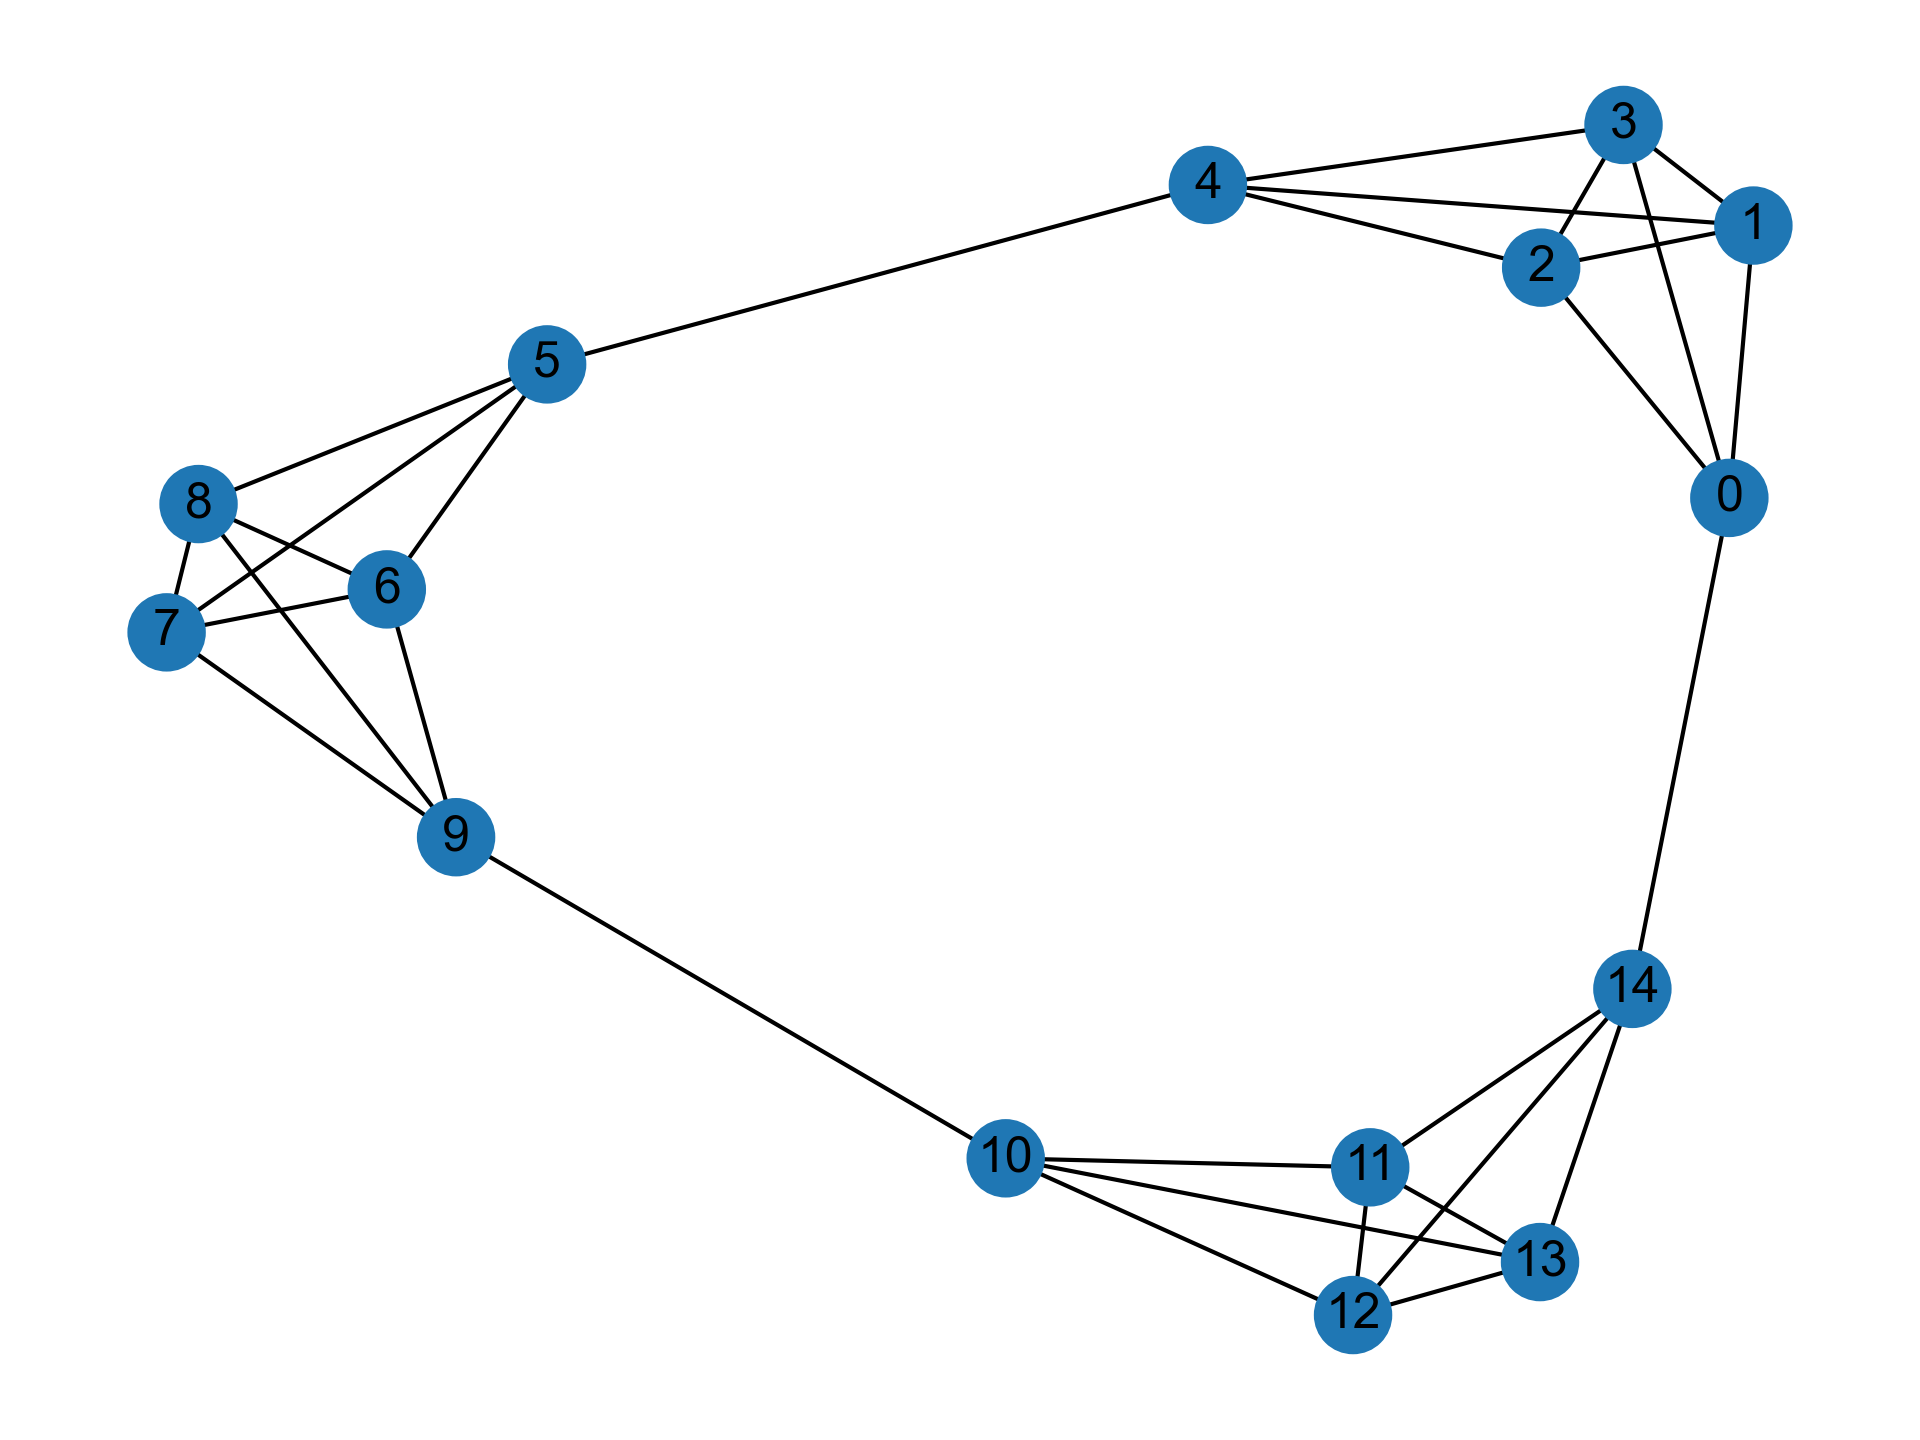
\includegraphics[width = \textwidth]{chapter_notebooks/chapter_2/figures/modular_graph.png}
	\label{fig:modular_graph}
\end{figure}

Why do we slow down at boundary nodes that lead to the adjacent module even when the local probability of that particular transition is the same as any other transitions? Understanding this particular property of human behavior may provide deeper insights into the kind of representations that lead to global-scale structure acquisition. Stimuli in tasks typically used in such statistical learning paradigms are either not meaningless or randomly assigned to each node -- the only difference between the boundary node and other non-boundary nodes is in context of the global structure of the graph. The event boundary literature (where boundaries are typically operationalized through explicit changes in context) suggests that boundaries alter the predictability of future events and this predictability leads to event segmentation \parencite{zacks2007event, clewett2019transcending}. Thus, in implicitly operationalized boundaries such as in serial reaction time tasks, the slowdown at the boundary node may imply a similarly increased uncertainty at boundary nodes leading to slowed responses. Prior work aimed at understanding human representation of graph structures indeed points to an increased `cross-entropy' between a learner's estimate of the transition probability and the true transition probability of the environment \parencite{lynn2020abstract, lynn2020humans, lynn2020human}. 

%In addition to being uncertain about the immediate next stimulus, participants are also uncertain about switching to a neighboring cluster or staying within the same cluster.

In particular, \cite{lynn2020human} show that algorithms of contextual representations such as the Successor Representation (SR) model in Reinforcement Learning \parencite{dayan1993improving, momennejad2017successor, gershman2018successor} or the associative learning based Temporal Context Model (TCM) can naturally lead to an increased cross-entropy for cross-cluster transitions relative to within-cluster transitions in modular graphs. In the current work, by using the framework of entropy as a proxy for an estimate reaction times in a modular graph we aim to 1) Experimentally test the predictions of these two models when exposure through the modular graph structure of is partial and 2) Identify which of the two models of representation best explain the observed data. 

\subsection{Representations of Temporal Context}

\subsubsection*{Successor Representation}
\label{successor-representation}

The Successor Representation (SR) model of reinforcement learning has been used as a model to understand the generalization of reinforcement learning behavior in large action spaces \parencite{dayan1993improving}. In recent work, the SR model has also been shown to be a reliable model for explaining human decision-making behavior in multi-step environments. The model's \yk{mechanism of model-free, trial and error learning of transition probabilities and model-based learning of rewards} accurately predicts that humans are worse at adapting to changes in the transition probability of a learned environment than to changes in the end-point rewards \parencite{momennejad2017successor}. There has been further evidence of SR being represented in the Hippocampal cells which represent space \parencite{gershman2018successor, stachenfeld2017hippocampus}.

Briefly, the SR model represents each state in the actionable space as a vector of predictive representations. For an environment of $N$ discrete states, the SR matrix $M$ of size $(N X N)$ maintains expected future visits to a given state from each state. Specifically, element $M_{i,j}$ of the matrix represents the expected future visits to state $j$ from state $i$. This transition matrix is learned over time based on the temporal difference error learning rule \parencite{sutton2018reinforcement}. For example, consider at a given point in time, $t$, an agent maintaining the SR matrix is in state $i$. The agent now moves to state $j$ out of the possible $N$ states. The $i^{th}$ row of the SR matrix is updated as follows:

\begin{equation}
	\hat{M}_{i,j} \leftarrow \hat{M}_{i,j} + \alpha[\delta(s_{t+1},j) + \gamma*\hat{M}_{s_{t+1},j} - \hat{M}_{s_t,j}]
\end{equation}

where $\delta(., .)$ equates to 1 if both arguments are equal otherwise it equates to 0. Thus, the matrix increases the probability of visiting a state $j$ from state $i$ if state $j$ is visited in the current experience and it decreases the probability of visiting all other states from state $i$. Parameter $\alpha$ is a learning rate parameter that determines how much of the previous estimate of visiting state $j$ from $i$ is factored into the current update. Parameter $\gamma$ is a future discount parameter that dictates how much in the future the agent sees -- specifically, a higher value of $\gamma$ indicates future visitations to state $j$ are weighed high in the current update.

\ac{For example, let's assume that the entire world (from the perspective of a participant) constitutes the 15 items they will see in the study. Now, as they start their experience of a random walk on the graph in Figure \ref{fig:modular_graph}, they will initially have no information about the transition probability structure. Thus, they will assign an equal probability across all possible transitions (i.e., $\frac{1}{15}$ between each pair of nodes/stimuli). Let's say they experienced a transition from node 1 to node 2. The prediction error for observed transition will be positive (example below)}:
\begin{equation}
	\begin{aligned}
		\Delta\hat{M}_{1,2} = 1 + \gamma*\hat{M}_{s_{2, 2}} - \hat{M}_{1,2} \\
		 = 1 + \gamma*\frac{1}{15} - \frac{1}{15} > 0
	\end{aligned}
\end{equation}

\ac{Similarly the prediction error for all transitions that were \textit{not} observed from node 1 will be negative (example below)}:

\begin{equation}
	\Delta\hat{M}_{1,3} = 0 + \gamma*\hat{M}_{s_{2, 3}} - \hat{M}_{1,3} \\
		= \gamma*\frac{1}{15} - \frac{1}{15} < 0
\end{equation}

\ac{Note that in the above equations, the model also accounts for a future transitions $M(2, 2), \& M(2, 3)$ while updating its expectation of transition $M(1, 2)$, and $M(1, 3)$ respectively. This way, any current transition impacts the expected trainstitions to the future nodes as well. \textbf{By allowing for transitions expected in the future to weigh in on current updates, this learned matrix allows for inferring for transitive properties in the graph structure.}}


\subsubsection*{Temporal Context Model}
The Temporal Context Model (TCM) was devised to explain the primacy and recency effects in human recall and recognition memory \parencite{howard2005temporal}. \ac{The TCM model assumes that the items or stimuli shown to a participant during a study phase through a sequential exposure maintain a temporal context \textbf{as a vector of activity of all stimuli in the experiment}. As new items get encoded, existing context from the previous items allows the new items to be bound to the previously seen items thereby sharing the temporal context}. Briefly, the TCM can be formalized as in \cite{gershman2012successor}:

\begin{equation}
	\begin{aligned}
		t_n = \rho * t_{n-1} + f_n \\ 
		\hat{M}_{i, j} \leftarrow \hat{M}_{i, j} + \alpha f_{n+1} t_{n, i}			
	\end{aligned}
\end{equation}

where $t_n$ is said to be a `context' vector for item $n$. The context drift parameter $\rho$ determines the proportion of the previous elements's context that gets incorporated in the current context. $f_n$ is a one-hot encoded vector for item $n$ \js{-- element of the $N$ item-vector $f_n$ is 1 for the item it represents and 0 otherwise}. The learning rate parameter $\alpha$ determines what proportion of the currently experienced state binds with the existing context. 

\ac{For a similar experience as described in the example for the SR model, the the TCM context vector $t_n$ is first updated based on the prior, existing context $t_{n-1}$. For the experienced transition from node 1 to 2 and assuming the current transition to node 1 came from node 0:}

\begin{equation}
	\begin{aligned}
		t_1 = \rho*t_{n-1} + 1  \\
		\hat{M}_{1, 2} = \hat{M}_{1, 2} + \alpha*1*t_{1,1} \\ 
	\end{aligned}
\end{equation}

\ac{Note that for a transition that is \textit{not} experienced, the cell $\hat{M}_{i, j}$ does not get updated as $f_{n+1}$ would be $0$.}

The key difference between the two models of temporal context is two fold: (1) SR Relies on error-based learning whereas TCM relies on hebbian, associative learning and (2) Through the future discount parameter $\gamma$, SR also learns the predictability observing states in the near future based on the locally experienced transitions. This future discount parameter in SR thus allows the model to represent transitive associations as well  \parencite{gershman2012successor}. 

\subsection{Model Simulations}

\mh{The differences between the models stated above lead to differing representations of learned temporal structure when the models are exposed through the random walk in Figure \ref{fig:modular_graph}. \ac{\textbf{To preview, representations associated with boundary nodes carry more information in the SR than the TCM.}}}

\mh{Simulating the models described above can thus lead to an estimate of expected behavior from both these models. Differences in these expected behaviors thus allow us to generate experimentally testable hypotheses.} Figure \ref{fig:SR-TCM-model-simulations} shows the context matrix representation after the models have been simulated for a random walk through the graph structure in Figure \ref{fig:modular_graph} as a result of a random walk after 1000 trials for both models. \ac{The matrices of Figure \ref{fig:SR-TCM-model-simulations} represent the model predictions of context representations. Each row corresponds to a context representation of that node (of the 15 total nodes). The `activity' levels in each cell indicated by the heatmap represent the relative proportion of nodes that are active when a particular node is visited.} 

\ac{\js{Parameters used in the simulations shown in Figure \ref{fig:SR-TCM-model-simulations} were determined by a Representational Similarity Analyses style procedure \parencite{kriegeskorte2008representational}. Specifically, for a combination of parameters over a valid range, a distance matrix was computed \textbf{\ac{to represent}} an euclidean distance between each pairs of rows of the generated context matrix (SR or TCM). Parameters that maximize the correlation between this generated distance matrix and the true distance matrix (derived from transition matrix representing equal probability transitions across the connected edges in the modular graph of Figure \ref{fig:modular_graph}) were chosen via a grid search.}} 

\begin{figure}[!ht]
	\centering
	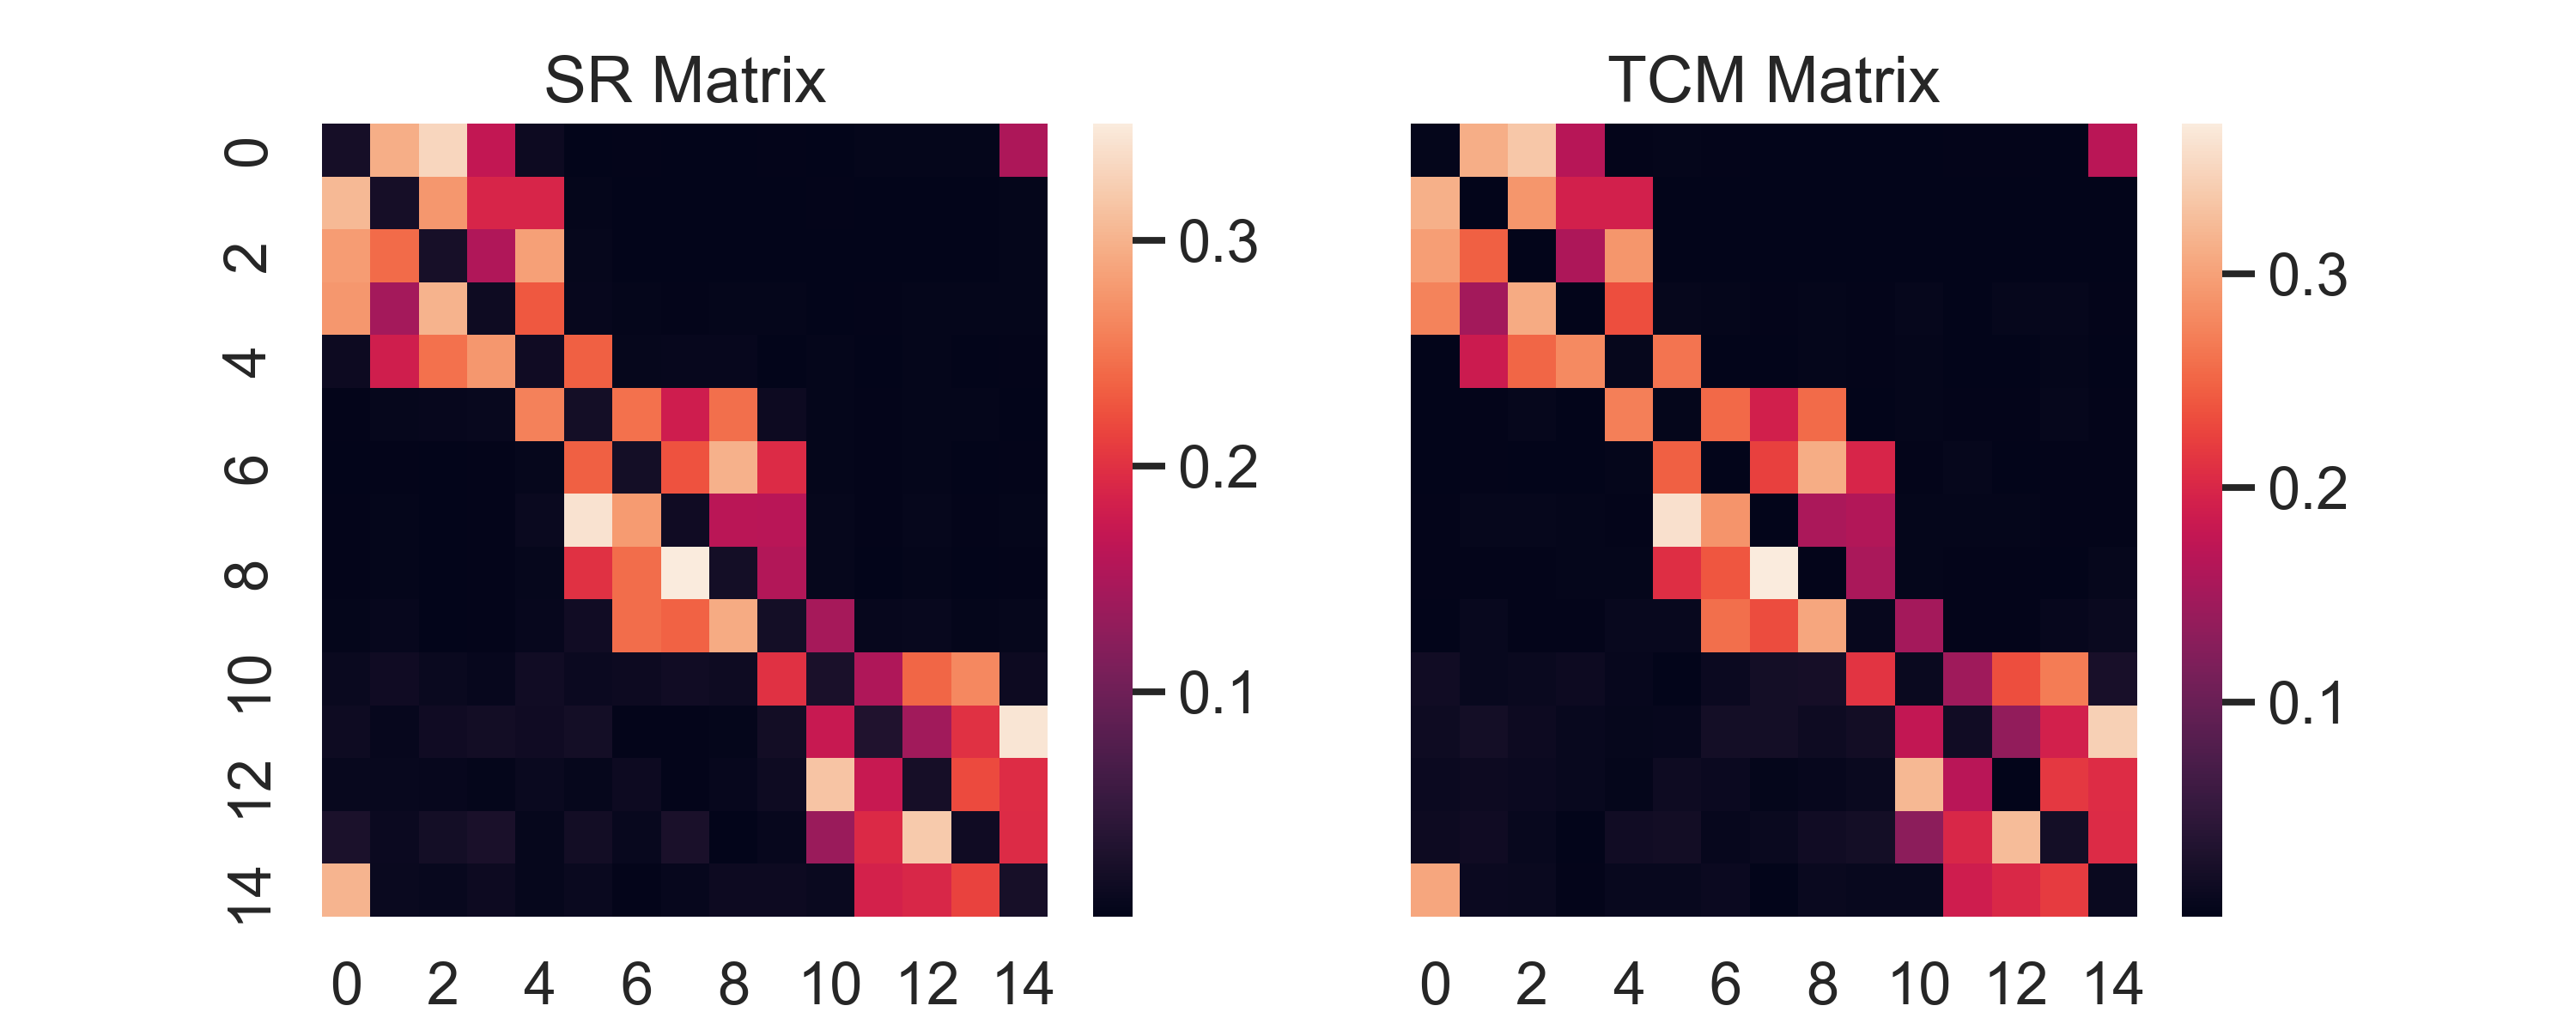
\includegraphics[width = 0.9\textwidth]{chapter_notebooks/chapter_2/figures/SR_vs_TCM_Matrices.png}
	\caption{Successor Representation and Temporal Context Model representations of context following a random walk through the modular graph structure.}
	\label{fig:SR-TCM-model-simulations}
\end{figure}


\ac{By using a behavioral measure of response times, previous work has shown that participants can acquire the global structure of the graph for a random walk. Particularly, as participants acquire knowledge of the underlying structure, their reaction times are slower in responses following a cross-cluster transition relative to a within-cluster transition \parencite{kahn2018network,kahn2018network,lynn2020abstract}.} To model this observed difference in reaction times and link them to the apparent differences shown in Figure \ref{fig:SR-TCM-model-simulations}, we apply principles of information theory. Specifically, we assume that response time for each stimulus is a function of the uncertainty in its surrounding context \parencite{fitts1964information}. Measures of information entropy have previously been used to explain RT differences between cluster transitions while traversing similar graph structures -- \ac{where higher entropy, which implies more uncertainty or more information available for a participant to process leads to higher response times \parencite{lynn2020abstract, lynn2020human,lynn2020humans}.} Formally, 

\begin{equation}
	\begin{aligned}
		RT(node) \cong Entropy(node) = \sum_{s' \in S} \hat{M}(s, s') * log(\hat{M}(s, s'))
	\end{aligned}
\end{equation}

where $M(s, s')$ is the context representation at node $s$. For SR, this expression evaluates to the expected future visits to state $s'$ from state $s$ whereas for TCM this expression evaluates to the extent to which $s'$ is activated as a result of $s$. 

As noted previously, a common indicator of participants having acquired the global structural knowledge is a slowdown in responses when the ongoing stimulus stream crosses a cluster (relative to transitions within a cluster) of the modular graph. Context representations can be used to model the cross cluster-transitions by computing a `surprisal' effect. For simulations, the surprisal effect is computed as the Jenson-Shannon distance between the context representations of two nodes. Formally, 

\begin{equation}
	\begin{aligned}
		RT(s \rightarrow s') \cong JS(s, s') = \sqrt[2]{\frac{D(M(s, .) || p) + D(M(s', .) || p)}{2}} \\
	\end{aligned}
\end{equation}

where $M(s, .)$ is the context representation of node vector $s$, $p$ is the point-wise mean of nodes $s$ and $s'$ and $D(M||p)$ is the Kullback-Leibler divergence between probability distributions $M$ and $p$. \ac{Jenson-Shannon distance thus scales with differences between the two context representations. Intuitively, since the representations of nodes 1 and 2 are similar (as shown in Figure \ref{fig:SR-TCM-model-simulations}), the Jenson-Shannon distance between these two nodes will be smaller than nodes 1 and 6. A direct measure or surprisal derived from the context matrix was also considered (See Figure \ref{fig:surprisal-sims} in the appendix for details)}

The formalization of observed response time differences due to surprisal (and node entropy) allows us to simulate expected reaction time distributions for novel walk types. Specifically, to understand the mechanisms behind acquiring the global modular graph pattern following a limited exposure \ac{(for example, infering the target store's organization via limited exploration over multiple visits)}, each model was simulated for random walk with lengths of 0, 3, 6, and 999. A random walk length of 0 translates to a completely random selection of one of the 15 nodes of the modular graph on each trial. Walk length of 3 and 6 translate to a random walk visiting 3 and 6 edges (4 and 7 nodes) respectively before being reset to a random node (similar to visiting the Target store in short bursts to purchase relevant items and checking out without visiting the entire store). Finally, a walk length of 999 translates to visiting 999 edges (with repetition) through their connections on the modular graph. \ac{Parameters of the simulations in Figure \ref{fig:SR-TCM-walklength-matrices} are determined through the same best-fitting RSA procedure described above.} 

\begin{figure}
	\centering
	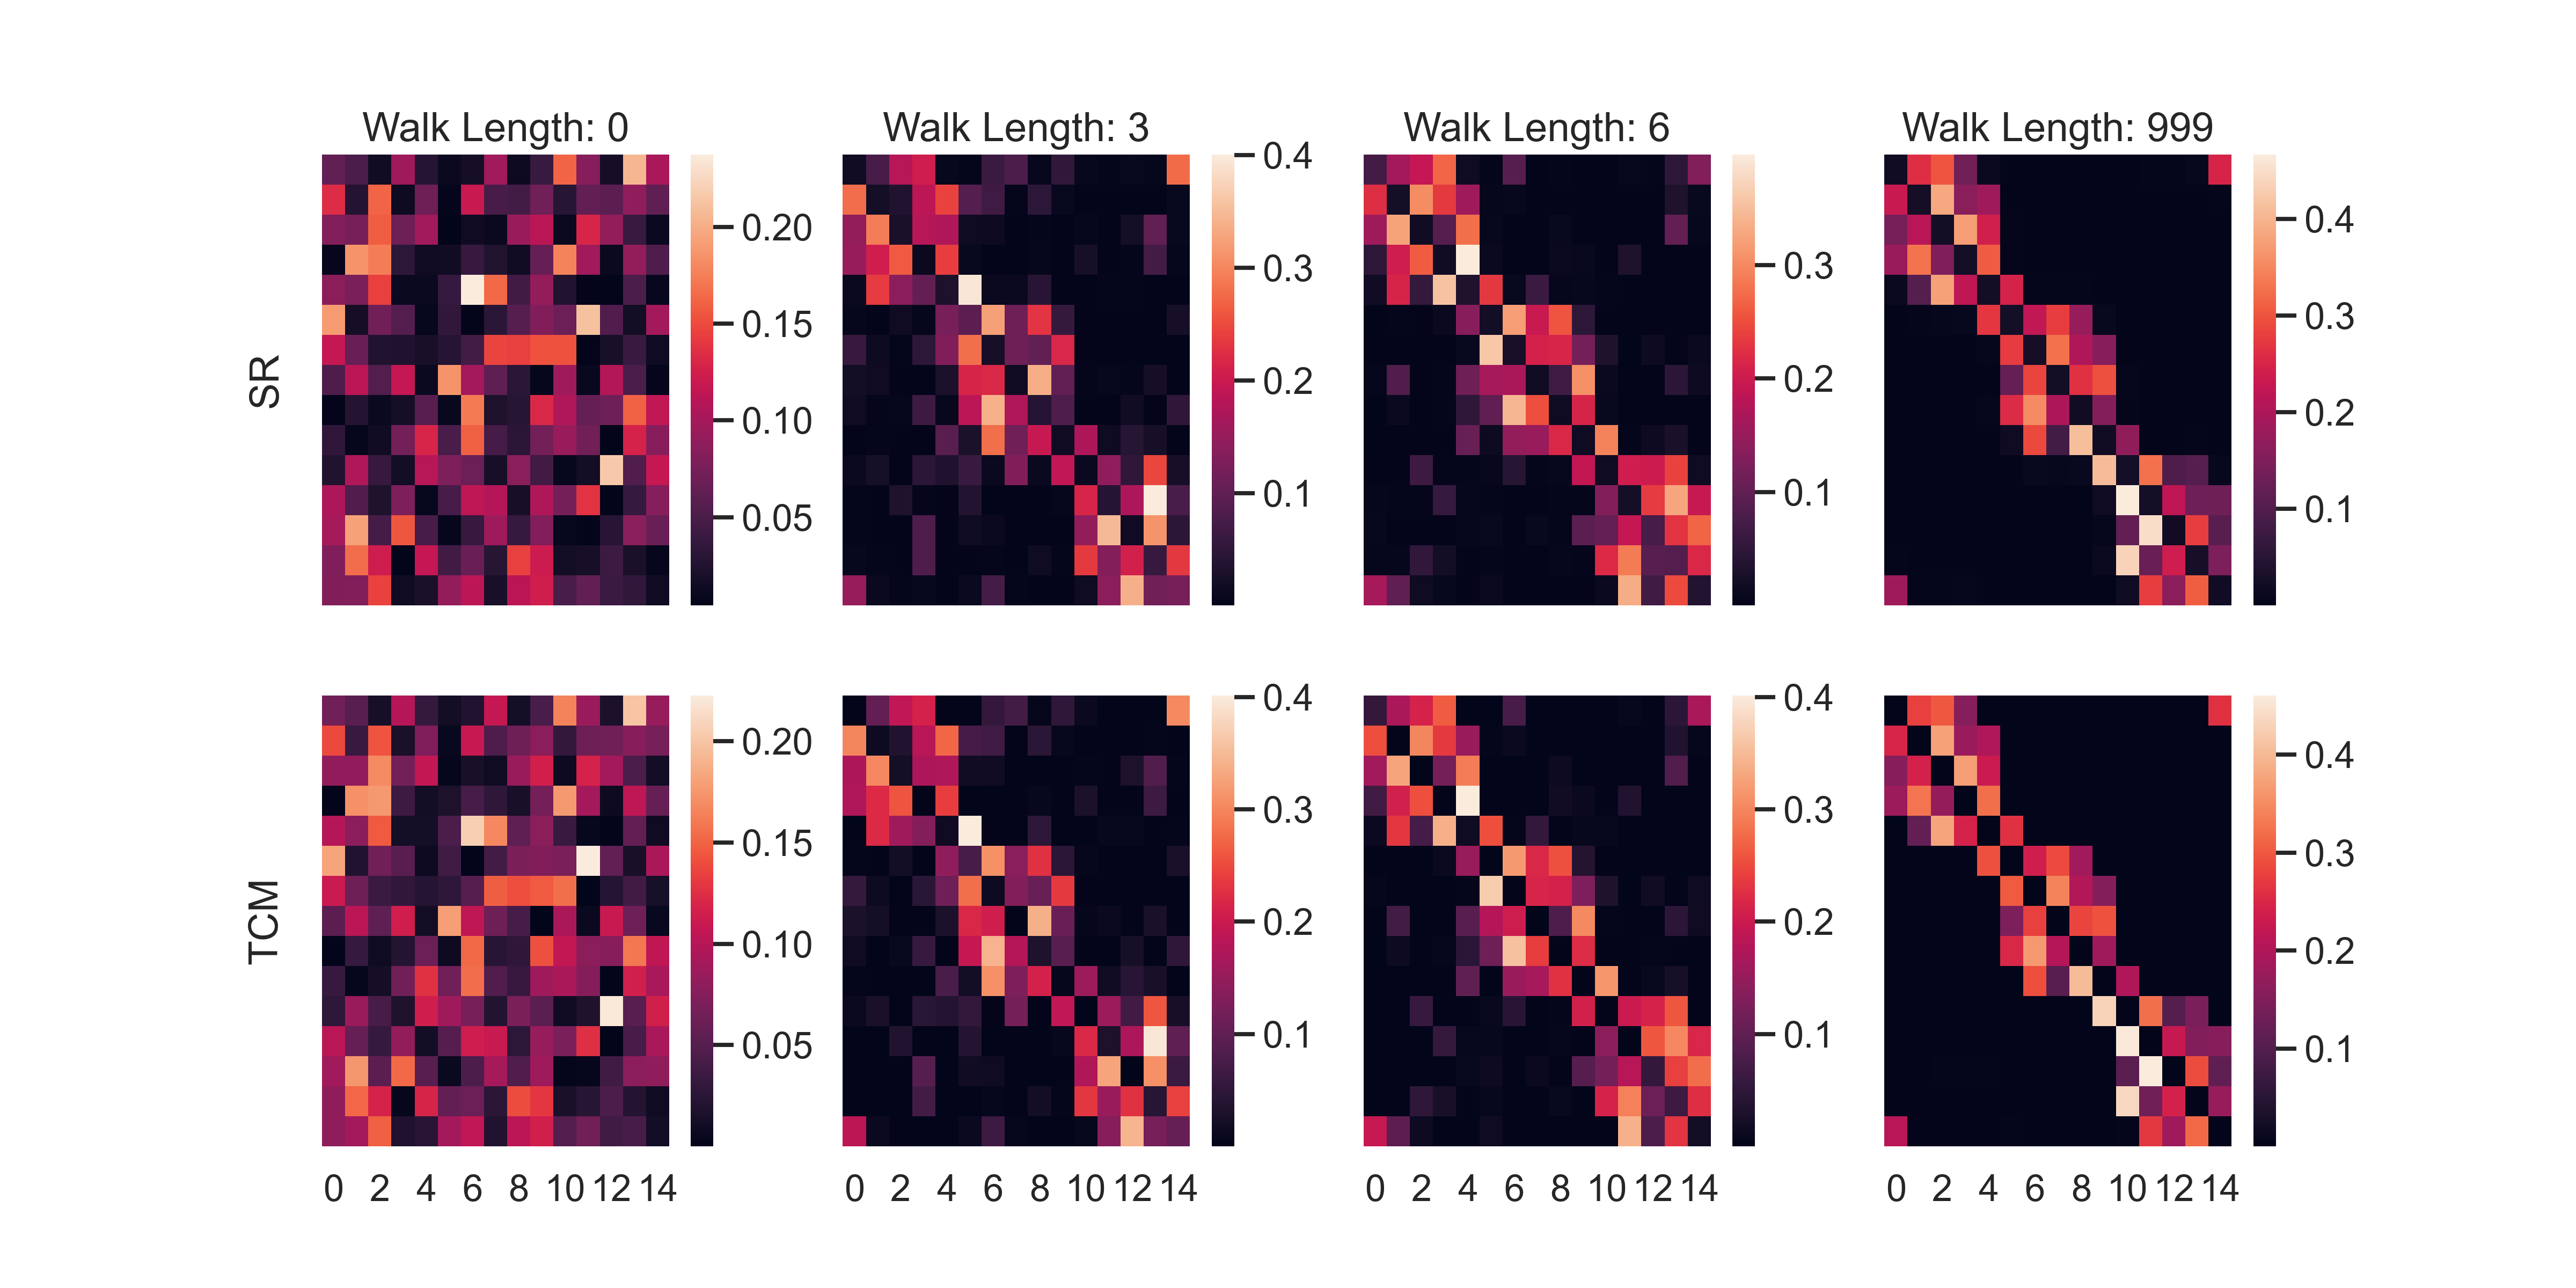
\includegraphics[width = \textwidth]{chapter_notebooks/chapter_2/figures/walk_length_SR_TCM_matrices.png}
	\caption{\ac{Example} model predictions of context representations for SR and TCM models across different walk lengths for \ac{one specific set of parameters}. Both models seemingly predict that the modular structure of the original graph is increasingly recovered with longer walk lengths.}
	\label{fig:SR-TCM-walklength-matrices}
\end{figure}

The acquisition of the global structure can be modeled using surprisal as has been done in previous research \parencite{lynn2020abstract,lynn2020humans,lynn2020human}. To investigate the differences between models for various walk lengths and relate to measurable response time differences,  for a subset of parameters in the valid range of 0 to 1, each model was simulated to produce a context matrix. Jensen-Shannon distance was computed between each pairs of nodes and averaged over cross-cluster pair and within cluster pairs. Simulation results below show the transition Jensen-Shannon distances over 100 simulations of the model for each parameter combination. For SR, `param\_a' is the learning rate parameter $\alpha$ and `param\_b' is the discount parameter $\gamma$. For TCM, `param\_a' is the learning rate parameter $\alpha$ and `param\_b' is the context drift parameter $\rho$. 
\begin{figure}
	\centering
	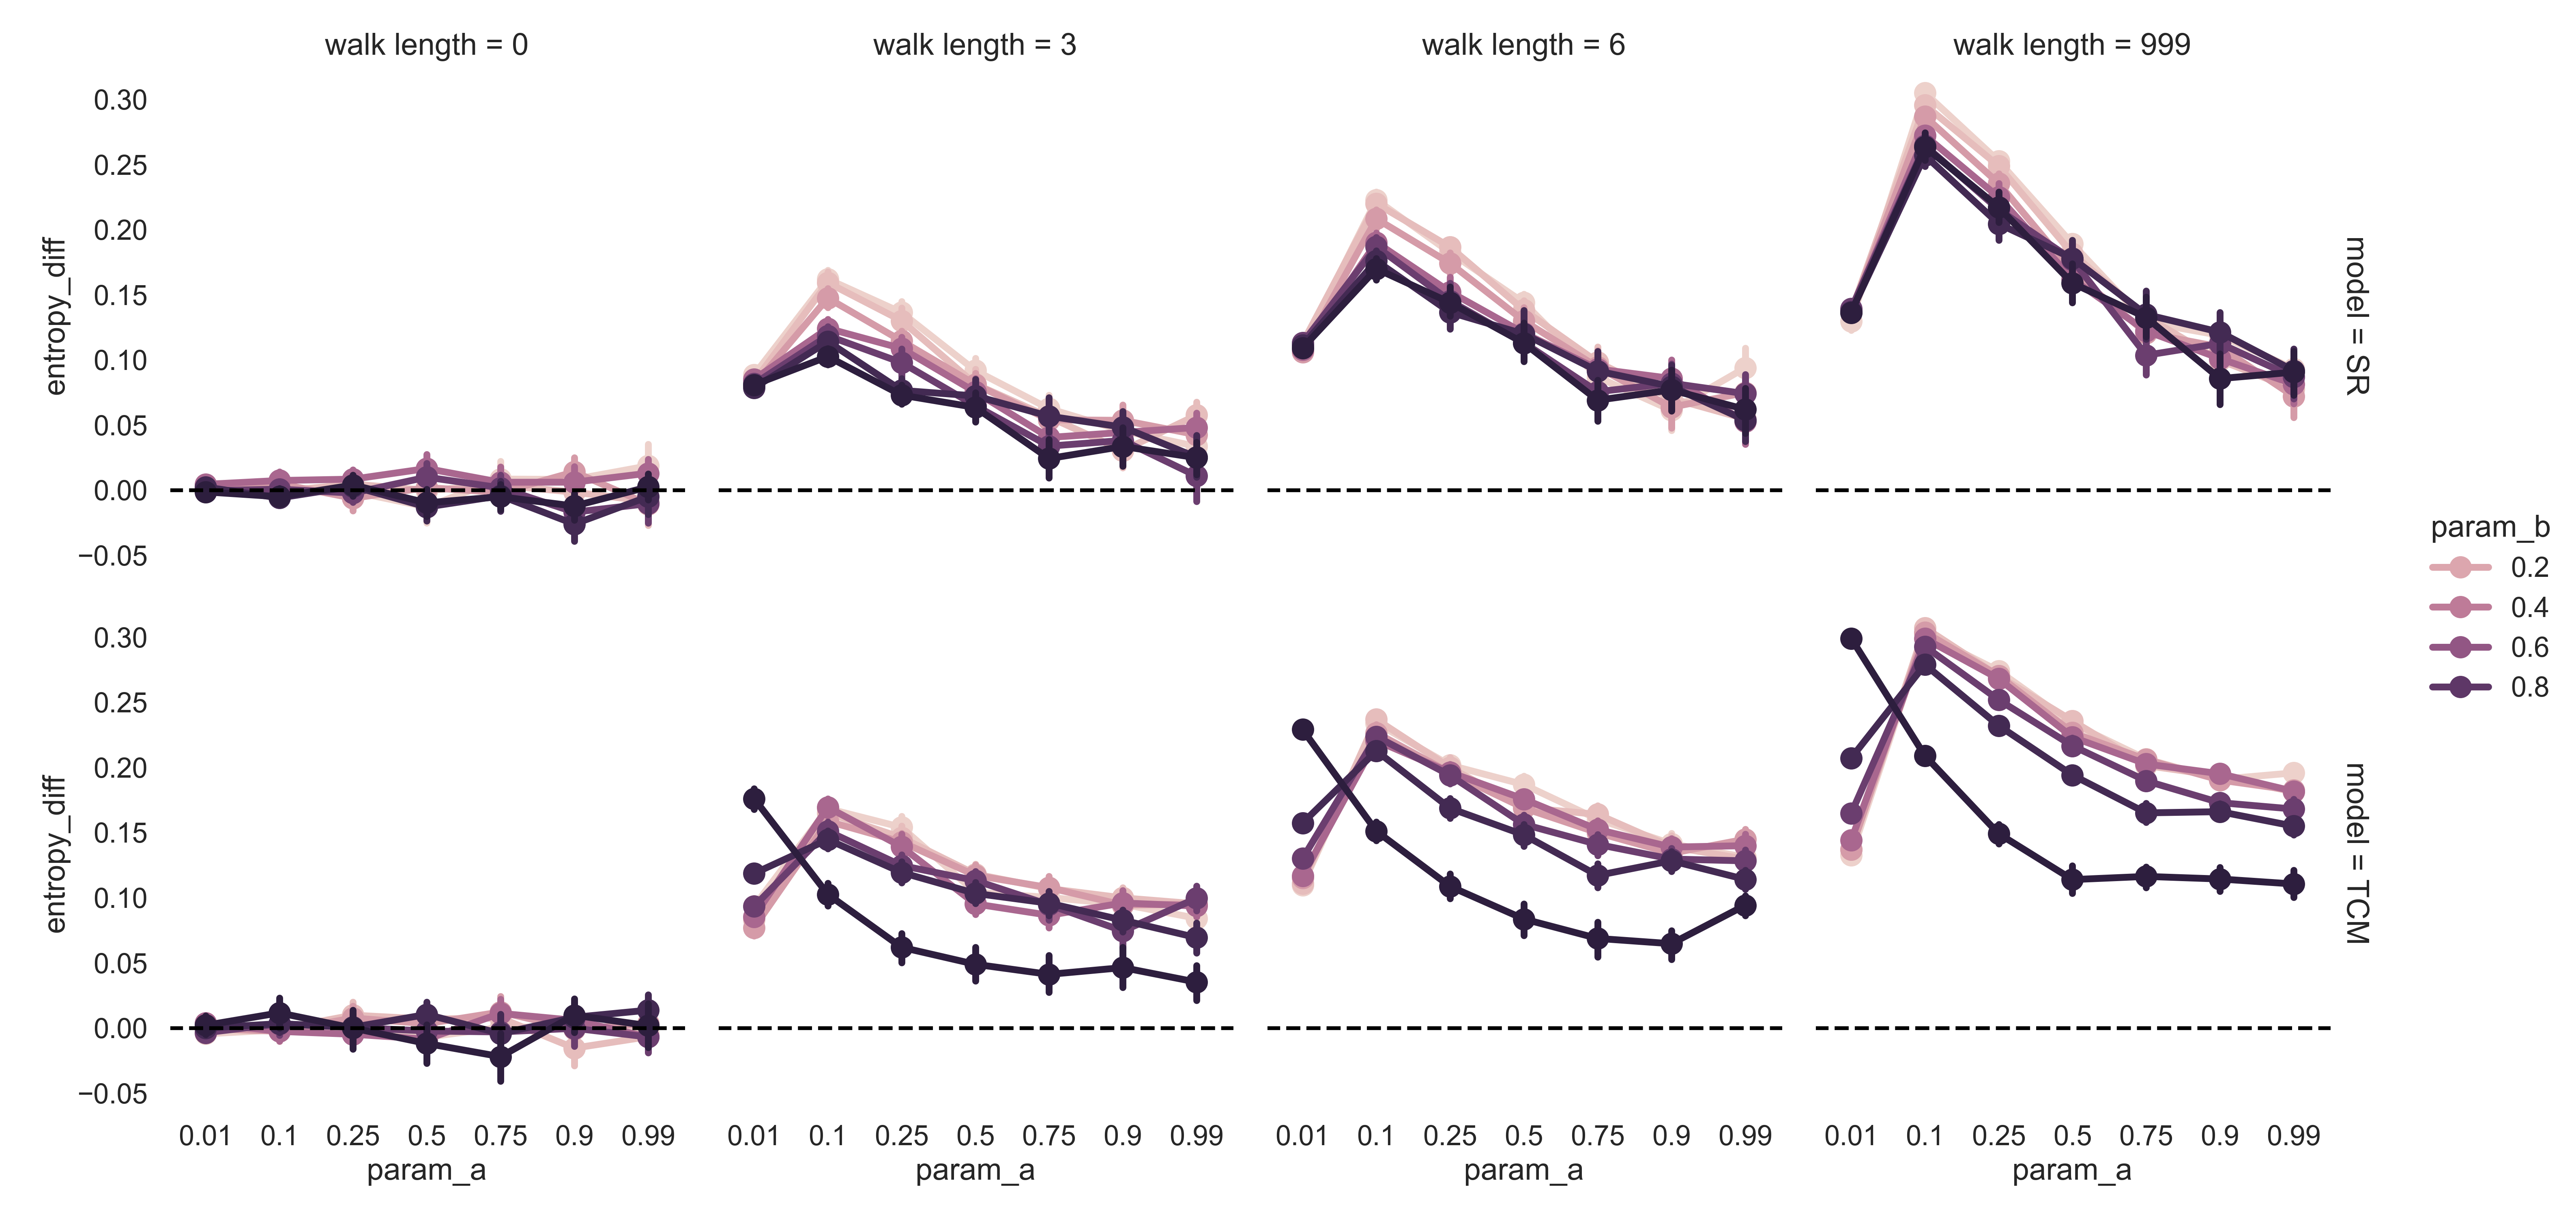
\includegraphics[width = \textwidth]{chapter_notebooks/chapter_2/figures/SR_TCM_boundary_nonboundary_jsdist.png}
	\caption{\yk{Simulated} model predictions for differences in surprisal comparing across cluster transitions to within cluster transitions across walk lengths \yk{for a range of possible parameter values}. Both models predict that cross cluster surprisal effect will increase with walk length leading to an increased reaction time.}
	\label{fig:SR-TCM-walklength-transition-sjdist}
\end{figure}

In Figure \ref{fig:SR-TCM-walklength-transition-sjdist} \ac{The Y-axis represents the difference in surprisal between boundary nodes and non-boundary nodes as measured by Jensen-Shannon distance. The X-axis represents the parameter $\alpha$ and different hues represent parameters $\gamma$ for the SR model and $\rho$ for the TCM model. Top row are predictions for the SR model and bottom row for the TCM. Columns represent predictions for different walk lengths.}. 

The figure thus shows that both context models predict an increased surprisal \ac{in cross-cluster transitions relative to within-cluster transitions} as walk length through the modular graph gets longer. As walk length increases, context associated with each node increasingly represents neighboring nodes. Since neighbors of the boundary nodes \js{\ac{are largely within the cluster of that boundary node, representations of boundary nodes becomes increasingly similar to that of the non-boundary nodes within the same cluster, and thus increasingly different than boundary nodes in the neighbouring cluster. Thus, crossing a cluster (from a boundary node to another) leads to an increased surprisal of having encountered a node that is representationally dissimilar to the previous node. On the other hand, non-boundary nodes within the same cluster get increasingly closer in their representations with other non-boundary nodes in that cluster. Thus transitions between non-boundary nodes within a cluster does not increase surprisal.}}

The two context models, however, differ in their predictions in the role of a boundary node. \ac{The Y-axis of Figure \ref{fig:SR-TCM-walklength-boundary-nonboundary-entropydiff} shows the difference in entropy between boundary nodes over a range of parameters (X-axis and hue) for both SR and TCM models (rows) across the 4 walk lengths (columns).} SR predicts an increased entropy in its representation of the boundary nodes with walk length relative to the non-boundary nodes for some values of the $\alpha$ and $\gamma$ parameters. On the other hand the TCM does not predict such increased in boundary vs non-boundary entropy differences. 

\begin{figure}[ht]
	\centering
	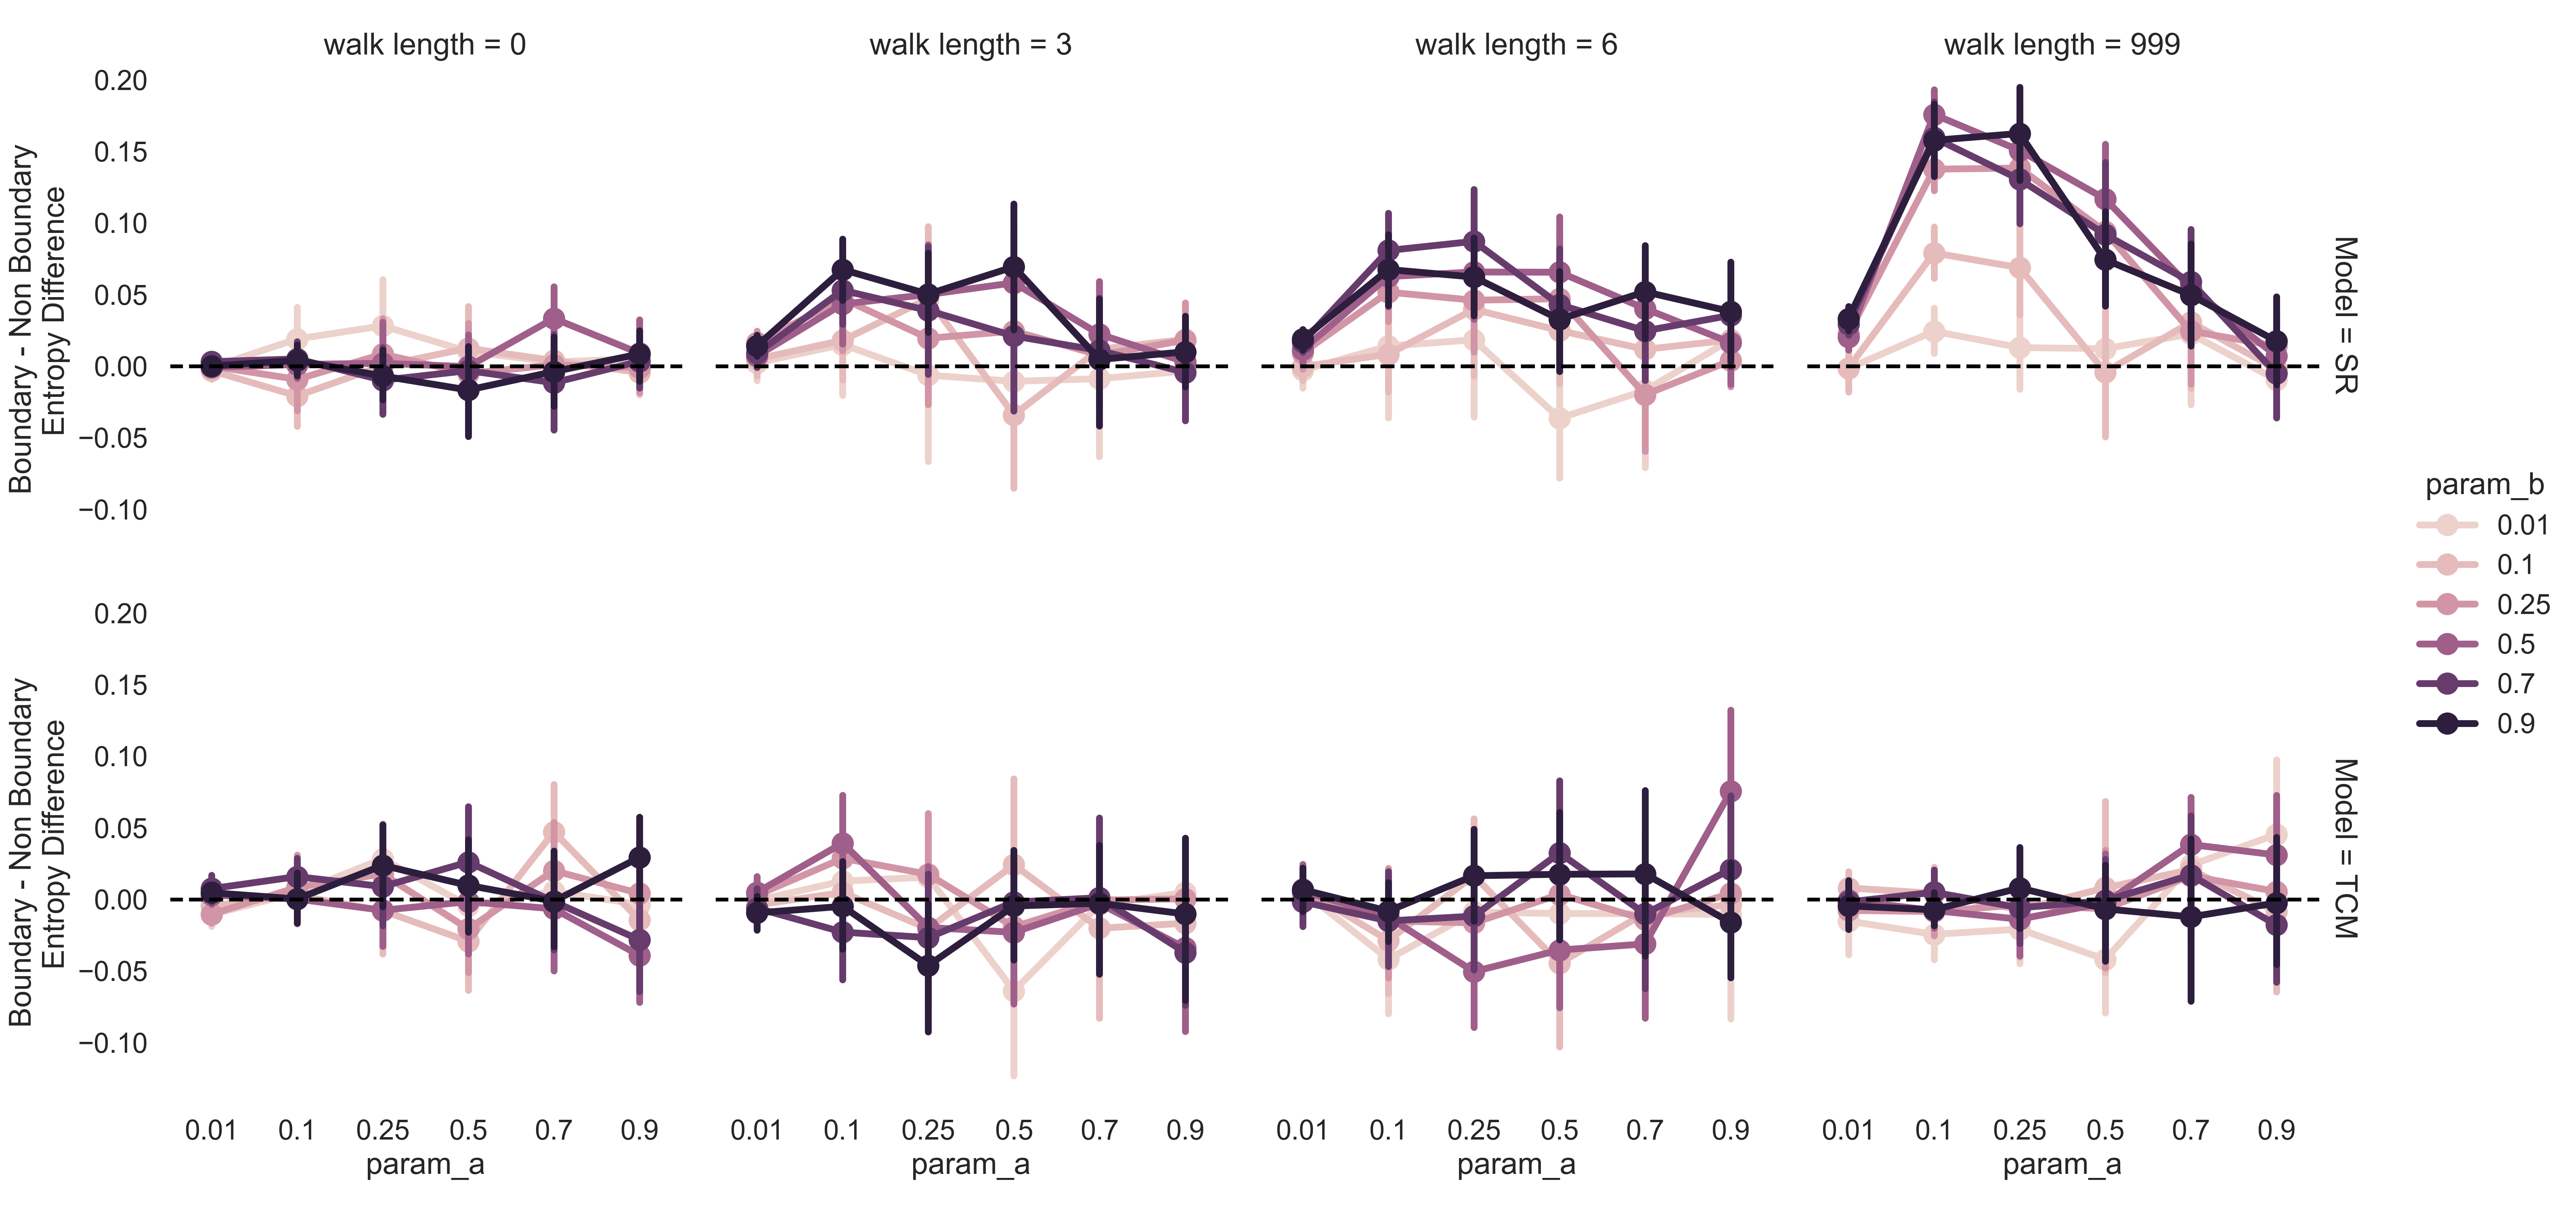
\includegraphics[width = \textwidth]{chapter_notebooks/chapter_2/figures/SR_TCM_walklength_boundary_nonboundary_entropydiff.png}
	\caption{\yk{Simulated} model predictions of differences between the SR and the TCM after different walk lengths for \yk{a range of possible parameter values}. SR predicts that entropy of boundary nodes will scale with walk lengths whereas TCM does not.}
	\label{fig:SR-TCM-walklength-boundary-nonboundary-entropydiff}
\end{figure}


The predictive nature of SR (as modeled by the future discount, $\gamma$ parameter) allows for a representation of nodes in the neighboring cluster to impact entropy on the boundary node of the current cluster that leads to that neighboring cluster. This effect is unique on boundary nodes of a cluster as non-boundary nodes of the second cluster are closer to the immediate neighbor of the current cluster (i.e. the boundary node that serves as an entry point to the second cluster). Since TCM is associative (as opposed to predictive), only nodes that are `active' in representation impact the representation of the just experienced node thereby. This mechanism thus reduces the impact of the non-boundary nodes in neighboring cluster. Rescaled heatmap in figure \ref{fig:zoomed-in-SRTCM-boundary-entropy} presents this effect.

\begin{figure}[ht]
	\centering
	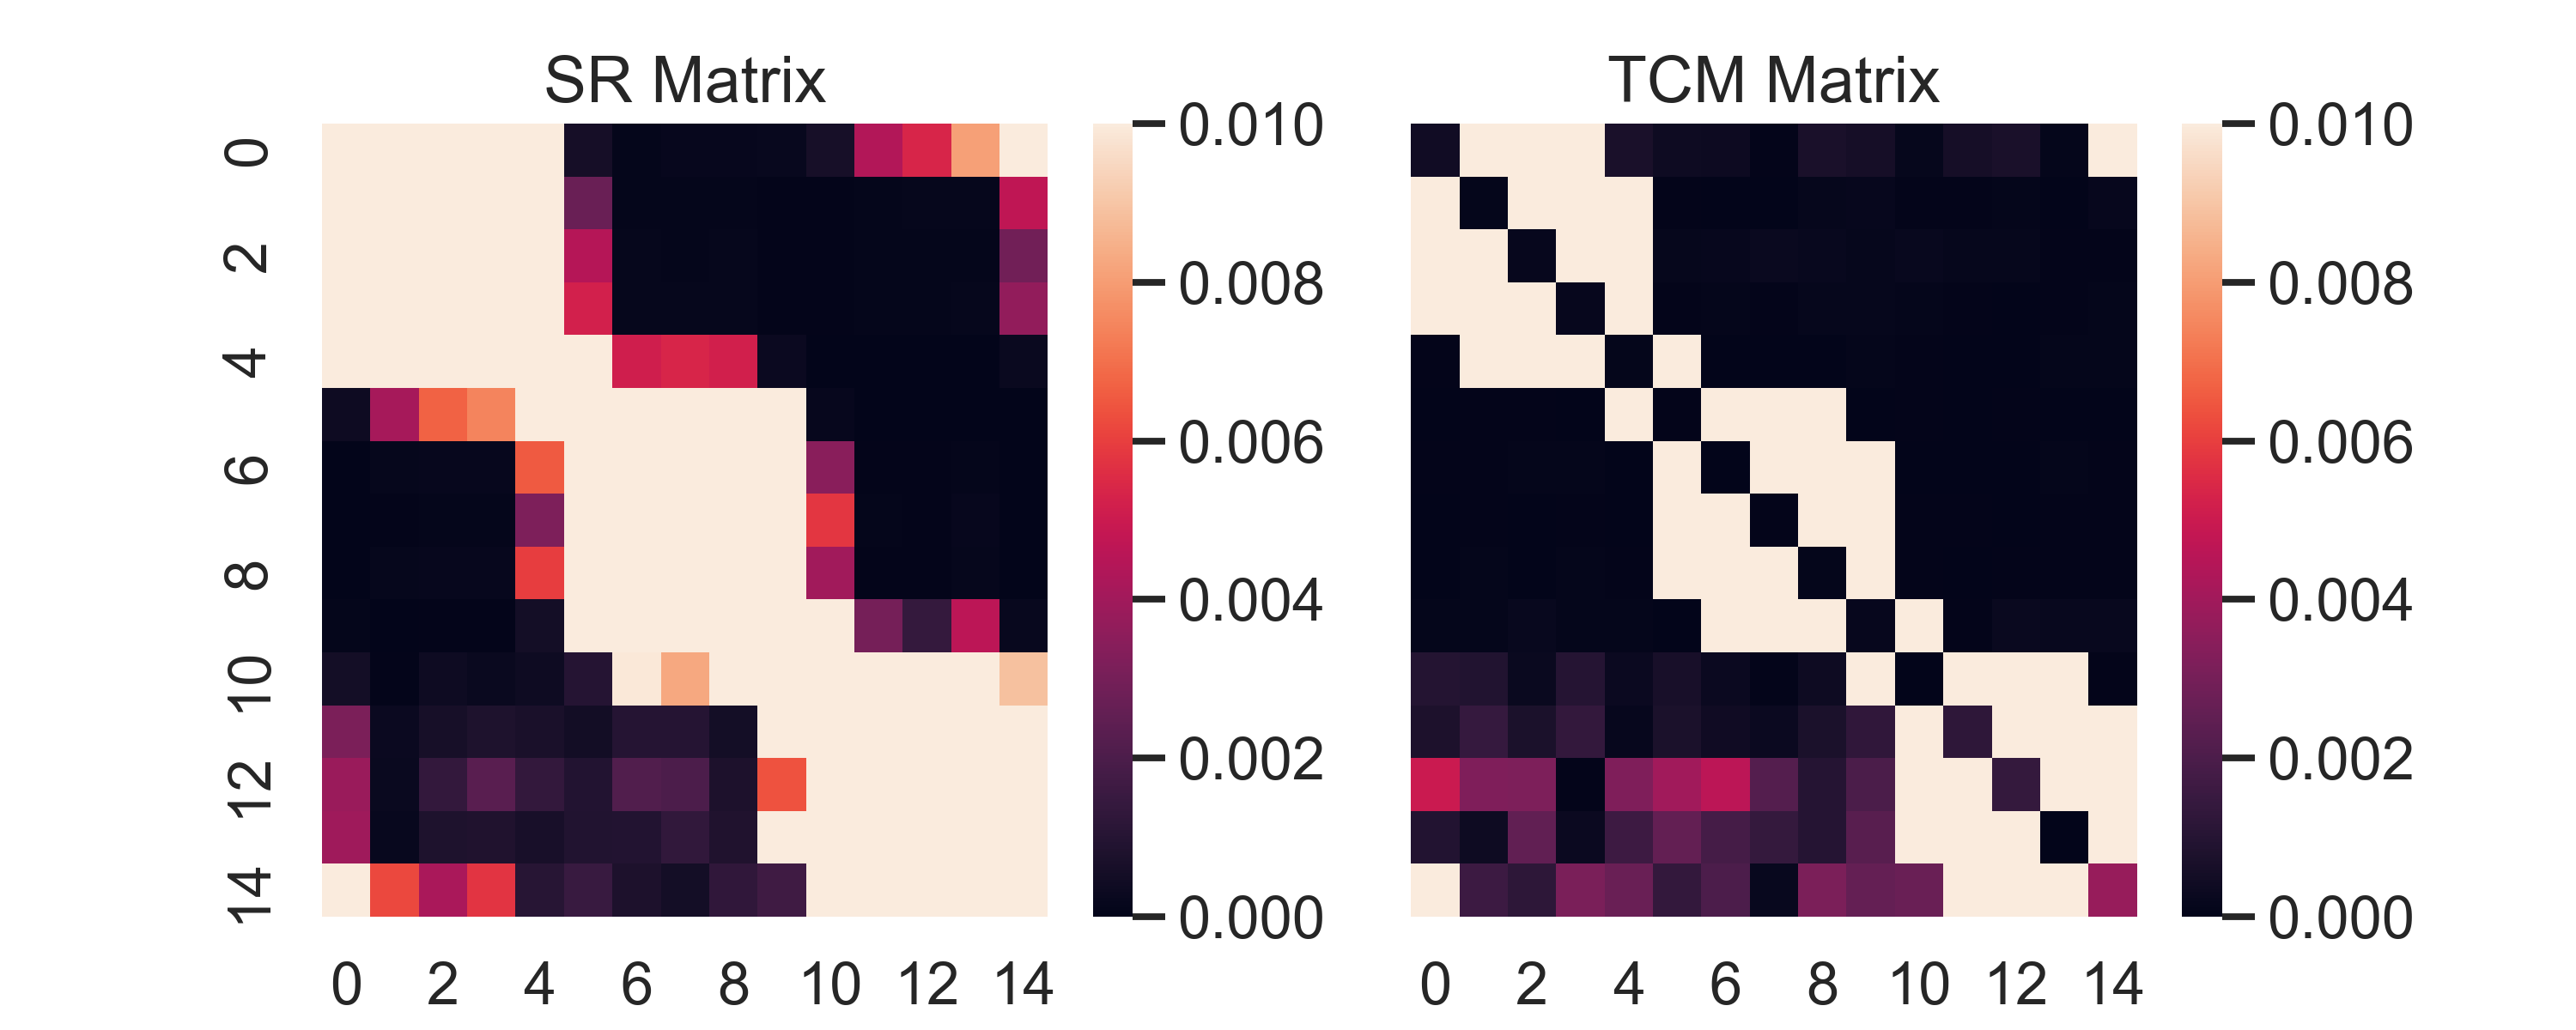
\includegraphics[width = \textwidth]{chapter_notebooks/chapter_2/figures/SR_vs_TCM_Matrices_zoomed.png}
	\caption{Rescaled SR and TCM matrices depict differences between context representations of the two models. Boundaries in SR incorporate more information than those in TCM.}
	\label{fig:zoomed-in-SRTCM-boundary-entropy}
\end{figure}

The SR-based predictive context representation in particular shows that boundary nodes carry more information than non-boundary nodes whereas the associative context representation does not produce this effect. \footnote{The activity in the lower third of both matrices is due to recency; while these are interesting patterns, and seem to indicate that SR can account for the recency effects in memory which was the primary motivation behind introduction of the TCM \parencite{gershman2012successor,howard2005temporal}. Investigating recency effects in this implicit statistical learning context is out of scope for this dissertation.}

Thus, both SR and TCM models would predict slow down in cross-cluster transitions relative to within cluster transitions, and that this slow down will increase with walk length. However, predictive context representations through SR are unique in predicting the scaled slow down at boundary nodes with random walk length, \textit{independent} \js{of where the boundary node has been visited from but as a result of the boundary nodes' inherent role in serving as a gateway between clusters}. While lack of a scaled slow down to boundary nodes does not invalidate the SR model (because some values of the parameters allows SR to not scale the slowed reactions with walk length), the presence of such a slow down provides evidence for predictive representations in such statistical learning tasks. The study presented next, thus tests this prediction. 

\section{Experiment 1: Testing Context Representations for implicit event boundaries}

\subsection{Methods}

\subsubsection*{Participants}
125 undergraduate students at the University of Massachusetts Amherst participated in this study for course credit. Data from 12 participants who did not complete the study was disregarded from further analyses. All study protocols were approved by the university institutional review board. \ac{Participant sample size was not pre-determined via a statistical procedure but was a rough equivalent of previous studies \parencite{kahn2018network,schapiro2013neural}}. \footnote{All inferences in this work are made in form of the probabilities of an effect as estimated via Bayesian analyses.}

\subsubsection*{Design and Procedure}

\ac{The general experimental procedure was similar to the one used by \textcite{kahn2018network}}. Participants were randomly assigned into one of four between-subject groups. All procedures for participants in all groups remained the same except for experimentally defined walk-lengths. Participants sat in an isolated room with an LCD computer screen operated by Windows 7. The experiment was designed using Psychopy \parencite{peirce2007psychopy}. 

As shown in Figure \ref{fig:exp1-design}, at the beginning of the study, participants were instructed to place their right hand on the computer keyboard such that their fingers aligned on the appropriate keys. On each trial, participants were presented with five grey boxes. One or two of the five grey boxes were highlighted using green borders. Participants were instructed to hit the combination of keys \yk{(simultaneously in cases where two keys were required to be hit)} corresponding to the highlighted boxes as fast as possible without making any errors. A trial did not end until participants hit the correct combination of keys. Participants were informed of their incorrect key presses and a trial where participants did not hit the correct combination of keys on the first try was marked as an inaccurate trial. The experiment lasted for 1400 trials, or 1 hour, whichever came first. To prevent fatigue, participants were given self-paced breaks after every 200 trials. Data from participants who did not complete all 1400 trials was discarded and not used for further analyses. At the end of the study, participants were debriefed about the research question of the study.

\begin{figure}
	\centering
	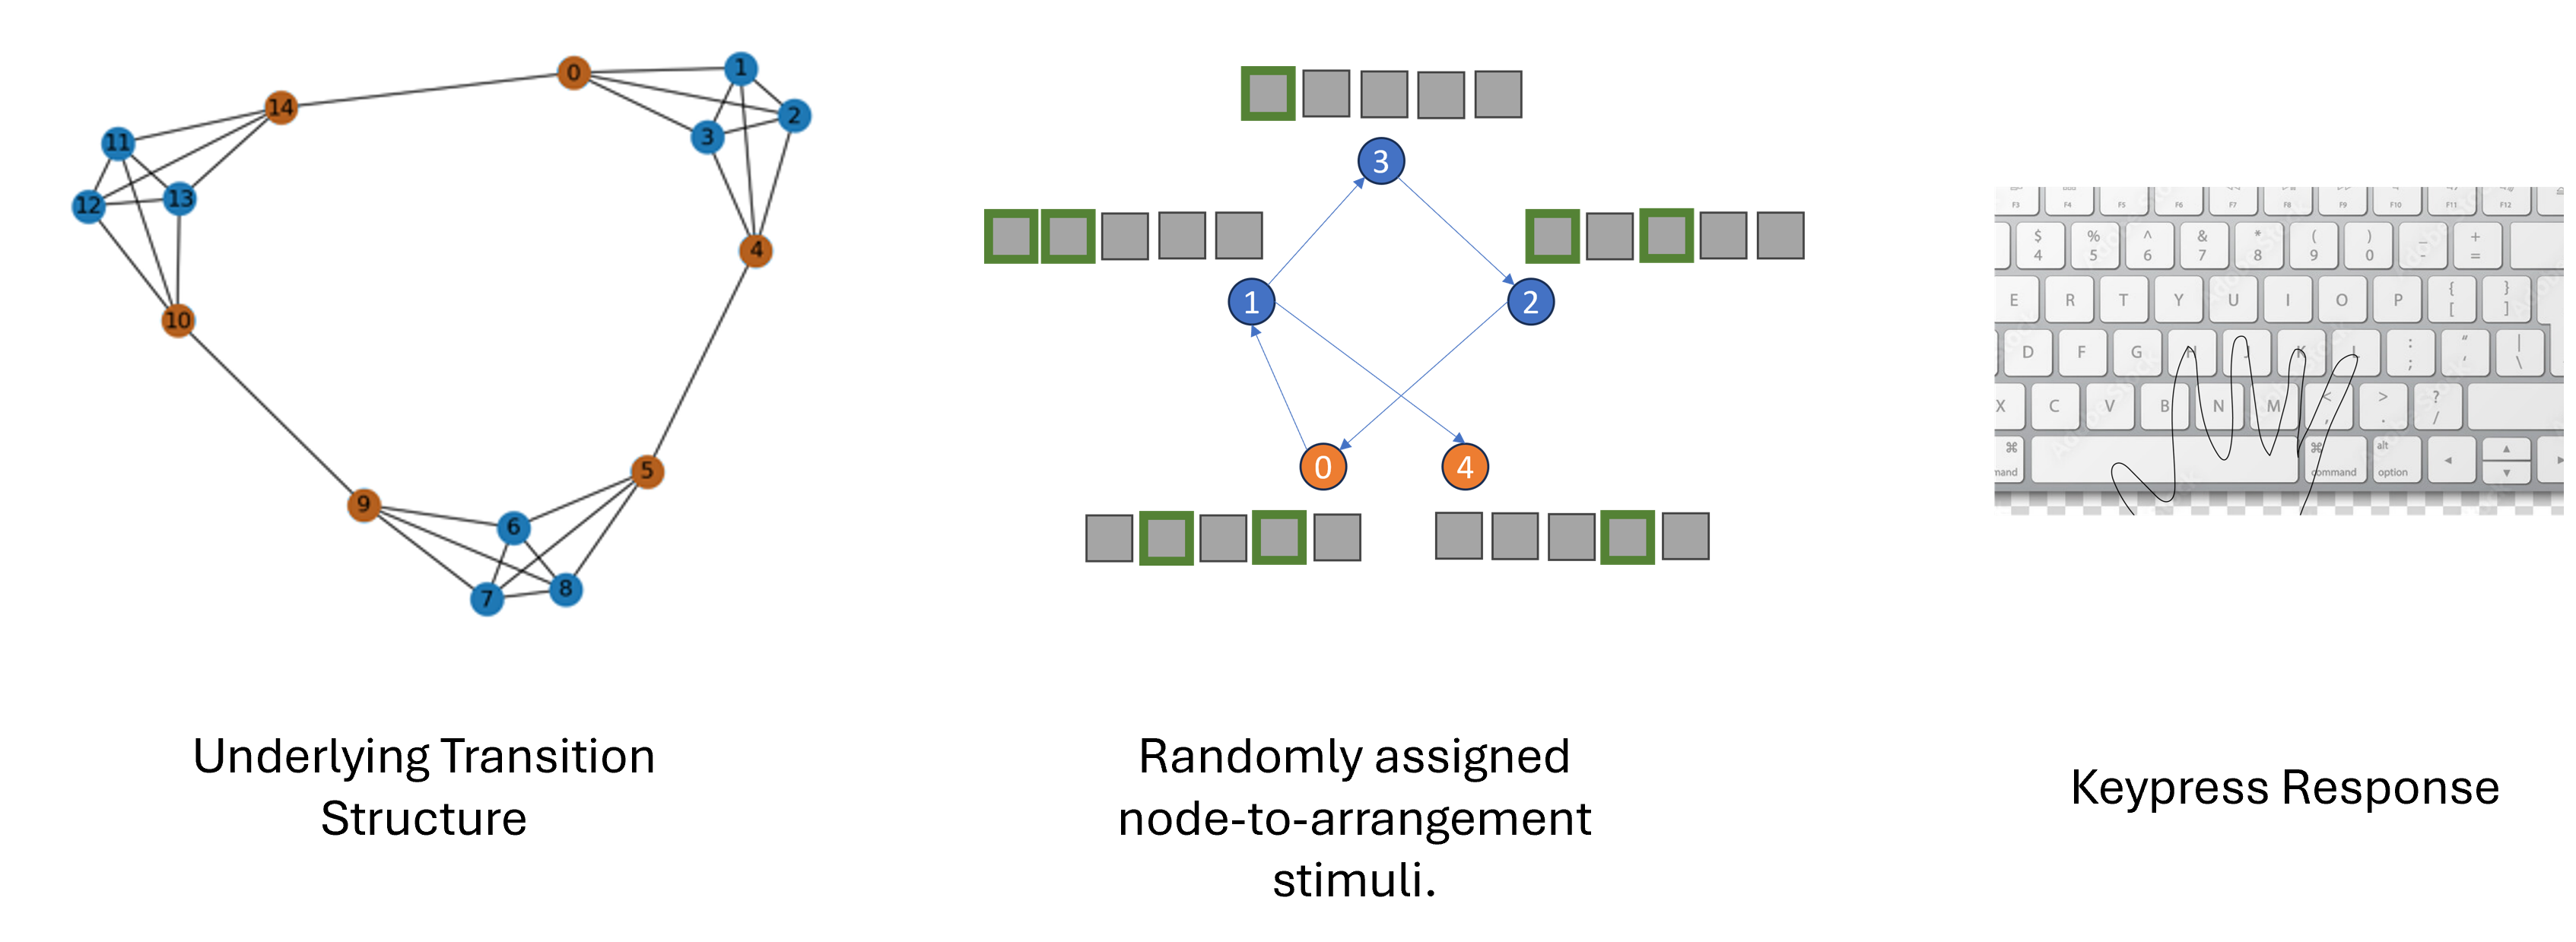
\includegraphics[width = \textwidth]{chapter_notebooks/chapter_2/figures/exp1_task_design.png}
	\caption{Task design for experiment 1. \textit{Left panel} modular graph used to generate random walks. \textit{Middle panel} Each node is randomly assigned to a combination of one or two highlighted boxes. \textit{Right panel} Participants place their hands on the keyboard as shown and are instructed to press keys that correspond to highlighted boxes.}
	\label{fig:exp1-design}
\end{figure}

Each of the 15 possible key combinations (where one or two of the grey boxes are highlighted) were randomly assigned to a node of the graph in \ref{fig:modular_graph}. Trial sequences were generated based on walk lengths. For all walk lengths, the first trial was selected at random. For walk lengths of 1399 (29 participants), the subsequent trials followed a random walk through the graph structure along the edges with edges connected. For walk lengths of 3 and 6, trials proceeded on a similar random walk for 3 (29 participants) and 6 (29 participants) edges respectively (thus visiting 4 and 7 nodes) before resetting to any of the fifteen nodes. Finally for random walk of length 0 (29 participants), each node of the 15 was picked with equal probability on each trial. 


\subsubsection*{Data Processing and Preliminary analyses}
All inaccurate trials (around 9.2\%) were removed from further analyses. Furthermore, accurate trials with response times beyond 3 standard deviations of the global response times (around 1.1\%) were removed from further analyses as well. In all, around 10\% of the total trials were discarded. 

\subsection{Results}
Table \ref{tab:exp1-rt-stats} shows the descriptive statistics \ac{(means, medians, and standard deviations)} of response time for each node and transition types \ac{aggregated over participants in each condition. The `Transition Type' column refers to the transition experienced immediately prior to a particular node where `within cluster' transition is the transition to a boundary or a non-boundary node from that same cluster and `cross cluster' transition is a transition to a boundary node from a boundary node of a neighbouring cluster. `Node Type' refers to the role of the current node in the graph of the left panel in Figure \ref{fig:exp1-design}.}

\begin{table}	
	\centering
	\caption{Response times descriptive statistics (in seconds) for experiment 1.}
	\label{tab:exp1-rt-stats}
	\begin{tabular}{lllrrr}
		\toprule
		 &  &  & \multicolumn{3}{r}{rt} \\
		 &  &  & mean & std & median \\
		transition type & node type & walk length &  &  &  \\
		\midrule
		\multirow[t]{4}{*}{cross cluster} & \multirow[t]{4}{*}{Boundary} & 0 & 0.954 & 0.565 & 0.786 \\
		 &  & 3 & 0.963 & 0.585 & 0.774 \\
		 &  & 6 & 0.973 & 0.594 & 0.785 \\
		 &  & 1399 & 0.990 & 0.596 & 0.802 \\
		\cline{1-6} \cline{2-6}
		\multirow[t]{8}{*}{within cluster} & \multirow[t]{4}{*}{Boundary} & 0 & 0.996 & 0.565 & 0.822 \\
		 &  & 3 & 0.980 & 0.598 & 0.787 \\
		 &  & 6 & 0.943 & 0.572 & 0.769 \\
		 &  & 1399 & 0.953 & 0.600 & 0.767 \\
		\cline{2-6}
		 & \multirow[t]{4}{*}{Non Boundary} & 0 & 0.963 & 0.565 & 0.790 \\
		 &  & 3 & 0.936 & 0.545 & 0.772 \\
		 &  & 6 & 0.985 & 0.616 & 0.790 \\
		 &  & 1399 & 0.932 & 0.592 & 0.747 \\
		\cline{1-6} \cline{2-6}
		\bottomrule
		\end{tabular}
	\end{table}
	

As expected, response times decreased with practice for all nodes in all conditions \mh{(Tables \ref{tab:first-last-blocks-3}, \ref{tab:first-last-blocks-6}, and \ref{tab:first-two-blocks-1399} for statistical comparisons)}. The median response times separated by transition type and node types are shown in Figures \ref{fig:rt-walklength-transitions} and \ref{fig:rt-walklength-nodes} respectively. \ac{Note that responses to Boundary node in Figure \ref{fig:rt-walklength-nodes} are a combination of within- and cross-cluster transitions.}

\begin{figure}
	\centering
	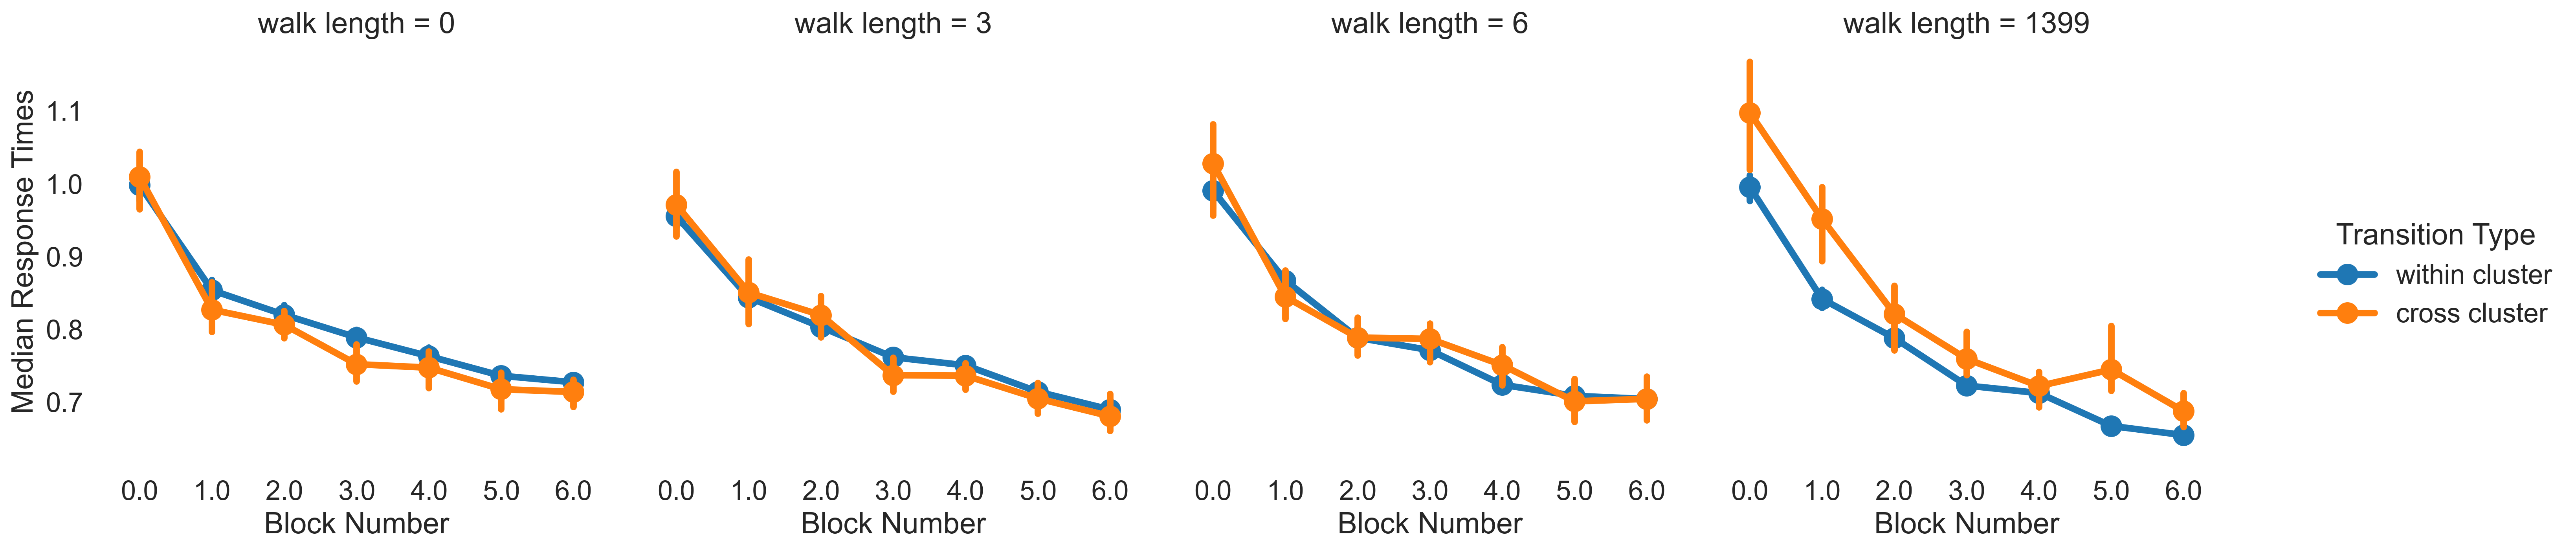
\includegraphics[width = \textwidth]{chapter_notebooks/chapter_2/figures/median_rts_transitiontype.png}
	\caption{Median response times \ac{at nodes following a transition} for each walk length separated by the type of transition.}
	\label{fig:rt-walklength-transitions}
\end{figure}


\begin{figure}
	\centering
	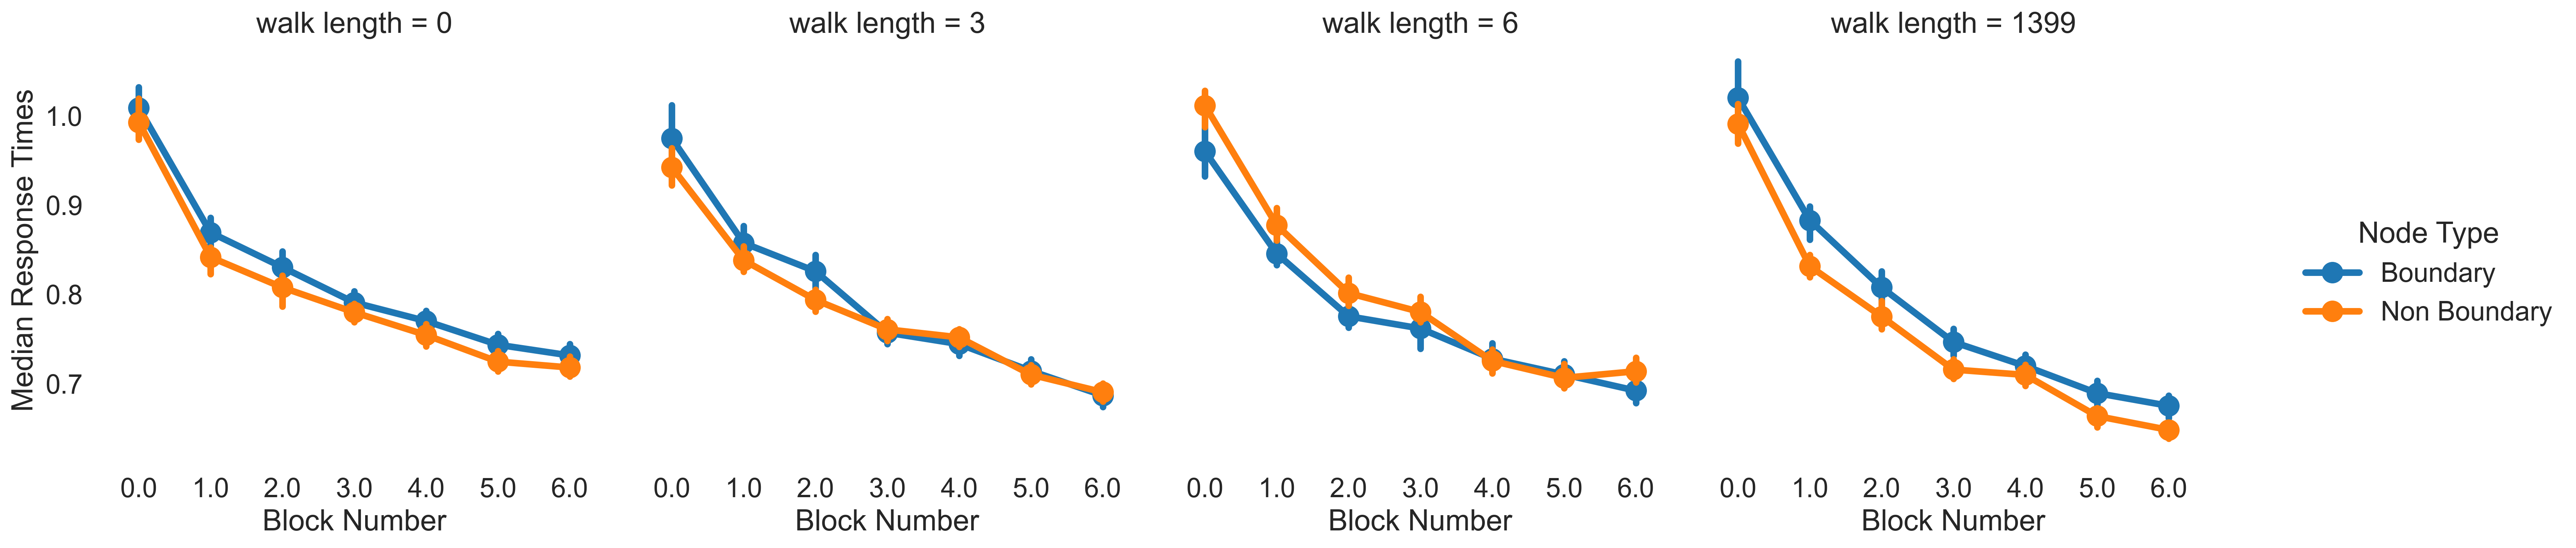
\includegraphics[width = \textwidth]{chapter_notebooks/chapter_2/figures/median_rts_nodetype.png}
	\caption{Median response times for each walk length separated by node types.}
	\label{fig:rt-walklength-nodes}
\end{figure}

Response time graphs show the overall pattern \ac{\textbf{expected from model simulations above}} -- cross cluster transitions are slower in longer walk lengths than within cluster transitions. Similarly, responses to boundary nodes are slower at longer walk lengths than responses to non-boundary nodes. 


\subsubsection*{Modeling}
The key question of interest is whether response times to boundary nodes slow down further \textit{after} accounting for slowdowns due to transitions. However, the effects of node type (comparing to non-boundary nodes) wll necessarily include effects of transition type since boundary nodes are accessed through both within cluster and across cluster transitions. Therefore, in order to isolate the effects of node type, response time differences between boundary and non-boundary nodes for within-cluster transitions were compared; thereby removing the effects of cross cluster transitions. Since transitions for walk length of 0 were random, this condition was also removed from further analyses. Similarly, all reset transitions in walk lengths of 3 and 6 \ac{(where the random walk ended and the subsequent node was picked between any of the 15 possible nodes)} which were \textit{not} a part of the random walk were discarded from further analyses \ac{to isolate the effect of the transition structure during a random walk (since nodes following resets do not follow the transition structure)}. 

Each block in the experiment consisted of 200 trials. Thus, by the end of the first block, participants in longer walk length conditions may have already experienced the graph structure sufficiently enough to acquire knowledge of the graph, thereby slowing down at the boundary nodes. While characterizing the entire 1400 trial learning curve \mh{\js{\ac{is ideal to measure the differences in reaction times of the critical transitions (non-boundary to non-boundary node compared with non-boundary to boundary node transitions), such linear model fit leads to the differences between reaction times at boundary and non-boundary nodes to map onto different parameters of the (see Appendix for a linear model of the entire learning curve) across different walk length making across walk length comparisons difficult}}}. Thus, to assess acquired patterns, the first two blocks of the data are compared using the following Bayesian model where standardized log response times were fit as a skewed normal distribution, separately for each walk length.

\begin{equation}
	\begin{aligned}
		node\ transition\ type : block \sim \mathcal{N}(0, 0.5) \\ 
		transition\ experience \sim \mathcal{N}(0, 0.2) \\  
		lag \sim \mathcal{N}(0, 0.2) \\ 
		\mu = node\ transition\ type : block + lag + transition\ experience \\
		\sigma \sim Exponential(1) \\ 
		skewness \sim \mathcal{N}(0, 3) \\ 
		log(RT) \sim Skew\mathcal{N}(mu, sigma, skewness)
	\end{aligned}
\end{equation} 

Where $node\ transition\ type$ is either non-boundary to non-boundary or non-boundary to boundary; block is 0 or 1, lag is the number of trials before which the current key combination was seen and transition experience is the number of times a particular transition leading into the current node was previously experienced. Figure \ref{fig:bayesmodel-firsttwoblocks} shows the Bayesian estimates of differences between walk lengths. \ac{The X-axis of the posterior histogram represents an estimate ofthe differences between response times at boundary nodes and non-boundary nodes in the second block (Block 1) after controlling for responses in the first block (Block 0) separeted by walk lengths of 3, 6, and 1399.}

\begin{figure}[h]
	\centering
	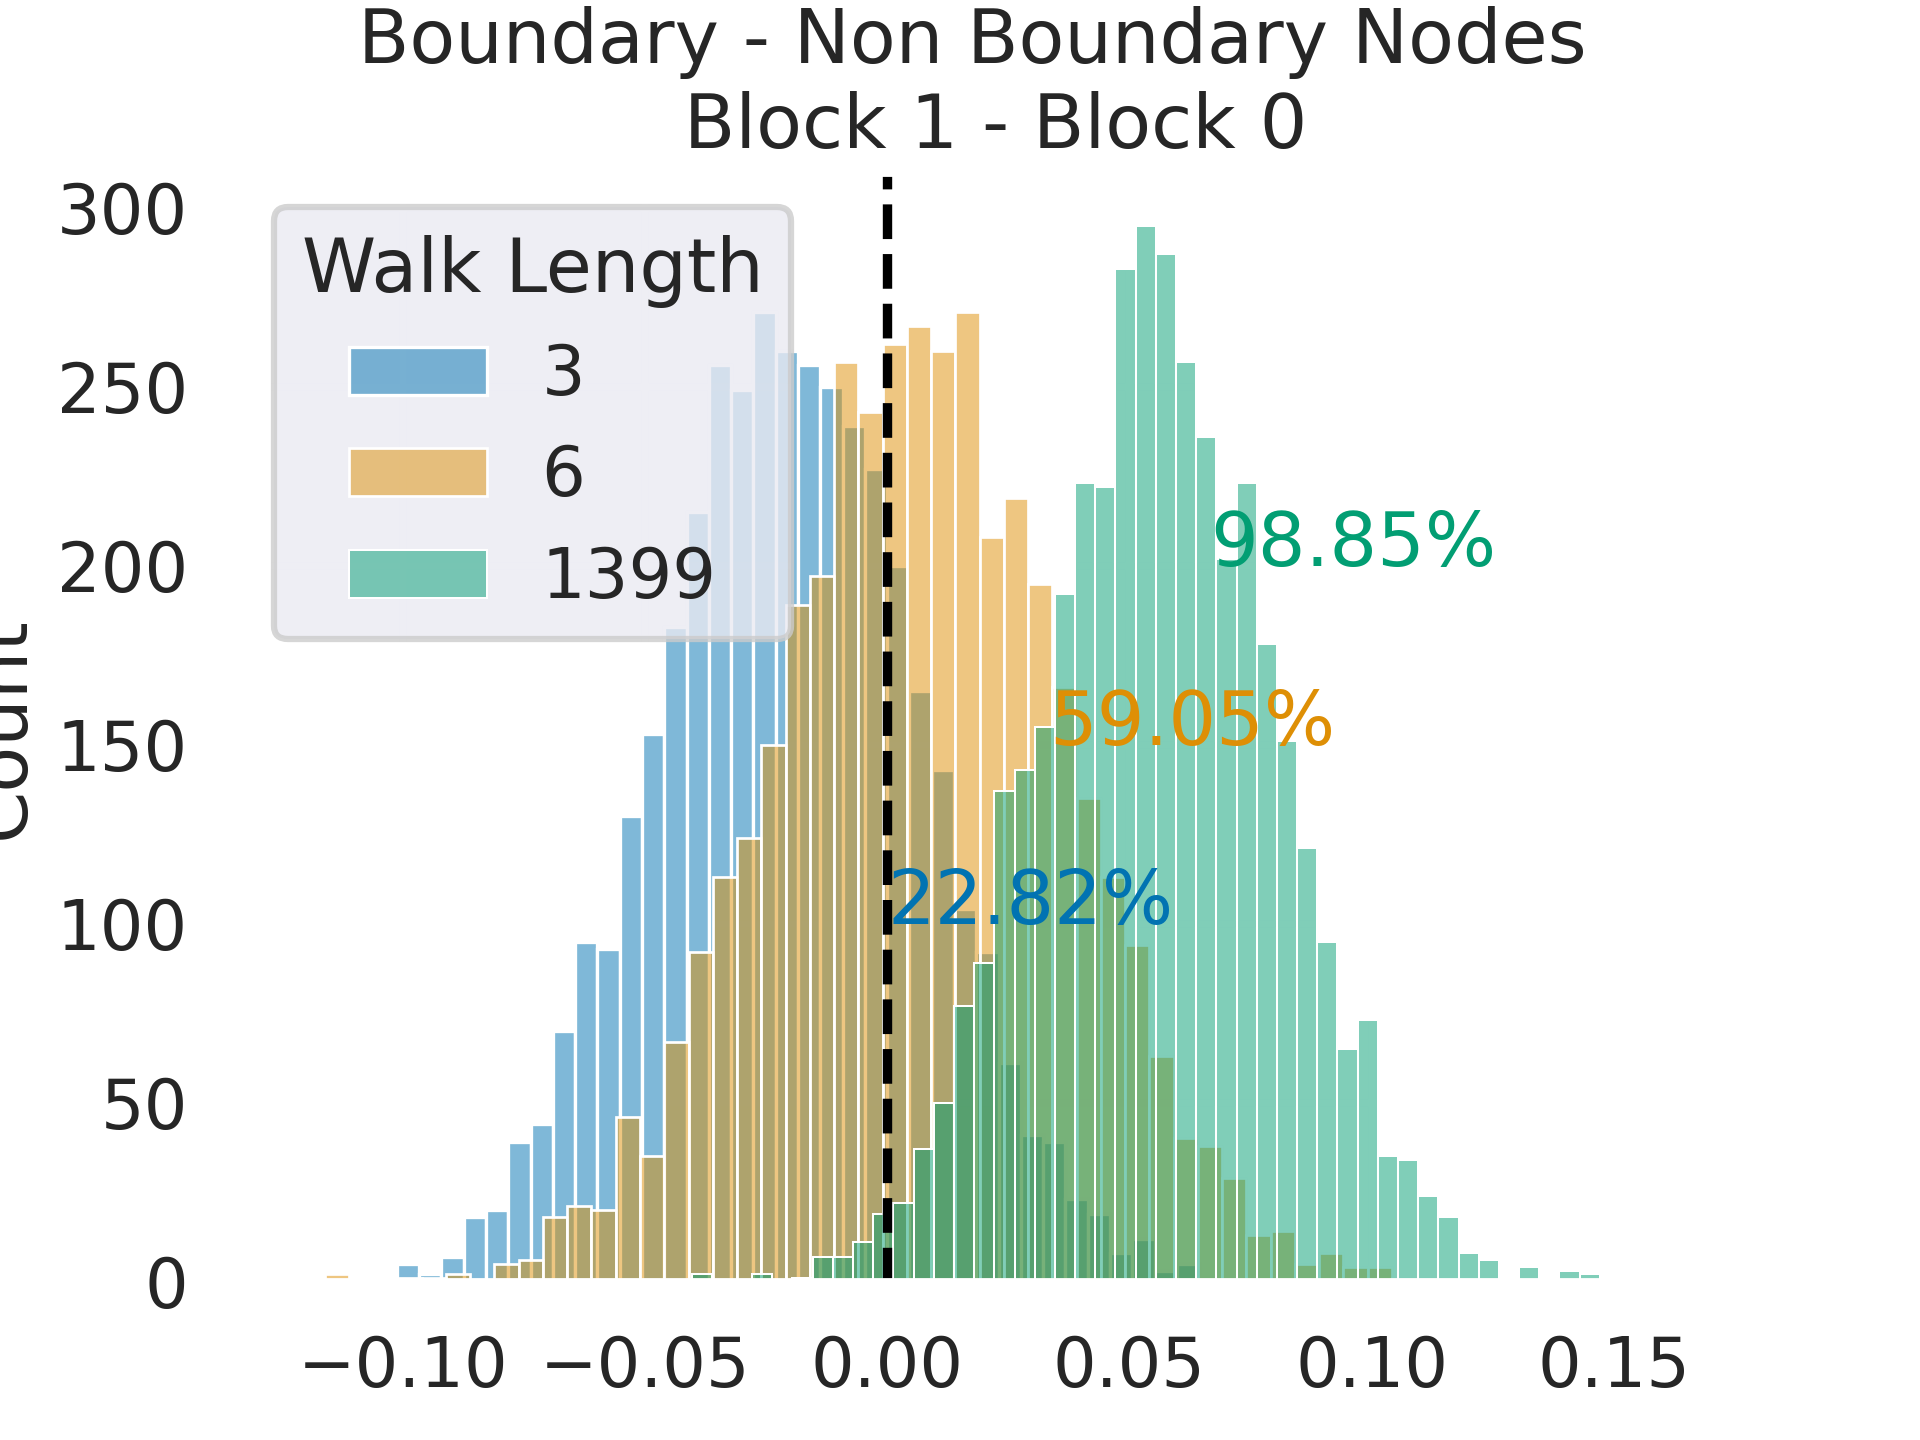
\includegraphics[width = 0.8\textwidth]{chapter_notebooks/chapter_2/figures/nb_b_diff.png}
	\caption{\ac{Estimated} differences in response times to boundary and non-boundary nodes when they are transitioned into from the same cluster (i.e. another non-boundary node). When accounting for the response times in the first block, as walk length increases, response times in the second block are increasingly slower to boundary nodes than non-boundary nodes.}
	\label{fig:bayesmodel-firsttwoblocks}
\end{figure}

In particular, participants in walk length of 1399 experienced the largest gains in response times of non-boundary to non-boundary transitions relative to those of non-boundary to boundary transitions from the first block to the second. As expected from the Successor Representation (SR) model, these gains were reduced for walk length of 6 and further so for walk length of 3 implying varying levels of structure acquisition depending on walk length. This pattern, which is uniquely expected in the SR model and not the TCM, thus provides support for predictive representations driving the formation of implicit event boundaries. 

\section{Discussion}

The primary aim of this work was to characterize the creation of implicitly operationalized event boundaries as a function of context representations. In particular, two models of context representations were contrasted: the associative TCM model and the predictive SR model. Both models express an increase in reaction time when crossing boundary nodes into a new cluster in the three-module graph structure (Figure \ref{fig:modular_graph}) as available context at boundary nodes across clusters drastically differs with each boundary node strongly representing events within its own cluster. However, the SR model \ac{expresses} the importance of boundary node as carrying additional information (measured by information theoretic entropy). The SR model predicts that as the `quality' of exposure (here operationalized by length of random walk) increases, the apparent importance of boundary nodes increases as well. 

To test this qualitative prediction of the SR (and thereby compare it with the TCM representation), a serial reaction time task was conducted with participants experiencing the modular graph at 4 different lengths of a random walk. As predicted by the SR, response times at boundary nodes slowed down the most for the longest random walk, and less so for shorter random walks. 

The experimental findings in this chapter thus provide support for maintaining a predictive representation of our environment \mh{and that associative, Hebbian mechanisms, are not enough to explain the observed data}. This error-driven predictive representation, which does not rely on explicit rewards, naturally leads to learning the statistical regularities in the environment and is thus crucial in informing our understanding of statistical learning and pattern acquisition. 

\mh{While SR is not unique in its expression of increased boundary information for a modular graph used in this work, other formulations (where increased boundary information is a result of erronous estimation of the transition probability) in prior work have been linked to closely follow the SR model \parencite{lynn2020abstract,lynn2020humans,lynn2020human}. Furthermore, this SR formulation allows us to use a neuro-psychologically plausible model in understanding pattern extraction and statistical learning \parencite{stachenfeld2017hippocampus,gershman2018successor,momennejad2017successor}. Finally, such predictive representations set stage for use of the SR (or SR-like) models over associative models to understand the broader work in event cognition and event boundaries \parencite{rouhani2020reward}.} 

In the current work parameters of the SR (or the TCM) model are not directly estimated as SR and TCM do not provide a direct measure of reaction times. While the assumption of reaction times scaling with increased available information (entropy) is logical, this assumption needs further testing. Future tests of such predictive representation should incorporate parameter estimation and hence also check the validity of the relationship between reaction time and information entropy. Similarly, a simpler model comparing two blocks was used to make inference in this task. More complex models (such as the exponential or the multi-rate state space models \parencite{savalia2024leap, smith2006interacting, mcdougle2015explicit}) should aim to characterize the entire learning curve to understand when participants start to acquire (and use) existing patterns. 

\mh{An SR based predictive representation, on its own is likely not sufficient to explain all patterns in the data. In some cases, participants may become explicitly aware of an existing structure, leading to a model-based reinforcement learning intervention on reaction times \parencite{momennejad2017successor} or constraints on working memory may require further considerations in how transition probabilities are learned \parencite{mcdougle2021modeling}. Future work should account for these possibilities in understanding the cognitive processes that underlie statistical learning.  Finally, findings presented in this work are limited to a single graph structure. Prior work has found that graphs of different topologies produce similar effects in cross-cluster slowdowns \parencite{karuza2019human} and future work should examine the modeling and experimental differences for a range of graph structures to assess whether findings in this work are dependent on the specific topological structure used.}  

\section{Conclusion}
The findings in this chapter provide evidence in favor of using predictive representations (as opposed to associative representations) to account for event boundaries that are operationalized implicitly. Findings in the current chapter do not distinguish between specific algorithms that lead to predictive representations; future work could contrast potential differences in these algorithms. It however remains unclear whether `boundary' nodes are truly so in context of event cognition -- the experiment presented in this chapter (and similar past literature) does not test whether stimuli at boundary nodes follow similar properties as stimuli at boundaries when events are operationalized through explicit context change. In the next chapter, I explore how such implicitly operationalized boundaries share properties with boundaries that are operationalized explicitly. 